\setcounter{secnumdepth}{4}
% Define colors
\definecolor{keywordcolor}{RGB}{255,0,0}
\definecolor{Classcolor}{RGB}{90, 90, 90}
\definecolor{Funcolor}{RGB}{191, 64, 191}
\definecolor{Logiccolor}{RGB}{51, 179, 255}
\definecolor{commentcolor}{RGB}{0,128,0}
\definecolor{stringcolor}{RGB}{163,21,21}

% Language definition
\lstdefinelanguage{CS}{
    language=C,
    morekeywords=
        {using, public, private, class, yield, return, new, if, else, out, try, catch, for, while, throw, foreach, in, using},
    morekeywords=[2]
        {ARRaycastManager, ARPlaneManager, GameObject, InventoryController, Vector3, ARPlane, Ray, RaycastHit, GetComponent, MeshRenderer, Quaternion},
    morekeywords=[3]
        {Start, Update, Awake, DelayedStart, IsPointerOverPlane, GetCurrentPlaneUnderGaze, SetPlaneColor, PlaceObjectOnDesk, ScreenPointToRay, SetActive, Euler, SetInventoryObject, Raycast},
    morekeywords=[4]
        {+, -, /, *, !, =, 0, 1, 2, 3, 4, 5, 6, 7, 8, 9, null, true, false}, % Define symbols as keywords
    morecomment=[l]{//},
    morecomment=[s]{/*}{*/},
    morestring=[b]",
    sensitive=true
}

% Listings settings
\lstset{
    language=CS,
    basicstyle=\footnotesize\ttfamily,
    keywordstyle=\color{keywordcolor}\bfseries,
    keywordstyle=[2]\color{Classcolor},
    keywordstyle=[3]\color{Funcolor},
    keywordstyle=[4]\color{Logiccolor},
    commentstyle=\color{commentcolor},
    stringstyle=\color{stringcolor},
    showstringspaces=false,
    breaklines=true,
    frame=single,
    numbers=left,
    numberstyle=\tiny\color{gray},
    tabsize=4,
    captionpos=b
}


\chapter{Feinkonzept und Realisierung}

\section{Entwicklungsumgebungen}
\subsection{Visual Studio 2022}
Visual Studio 2022 ist eine integrierte Entwicklungsumgebung (IDE) von Microsoft, die speziell für die Entwicklung von
Softwareanwendungen, Webanwendungen und Desktop-Anwendungen konzipiert ist. Es handelt sich um eine umfangreiche
Entwicklungsumgebung, die von Entwicklern weltweit für eine breite Palette von Anwendungsfällen eingesetzt wird.

\subsection{Unity}
Der Unity-Editor, entwickelt von Unity Technologies, fungiert als umfassende integrierte Entwicklungsumgebung (IDE)
und zentrale Arbeitsumgebung für die Konzeption und Umsetzung von 2D-, 3D-, Augmented Reality (AR) und Virtual Reality
(VR) Anwendungen und Spielen. Als Kernelement der Unity-Plattform spielt der Editor eine entscheidende Rolle in der
Entwicklung von Projekten, die auf Unity-Technologien basieren.

Die Funktionalität des Unity-Editors erstreckt sich über verschiedene Aspekte der Softwareentwicklung, angefangen bei
der visuellen Gestaltung von Szenen und Spielwelten bis hin zur Implementierung komplexer Logik und Interaktionen. Die
folgenden Abschnitte vertiefen die Schlüsselmerkmale und Funktionen des Unity-Editors, die ihn zu einem essenziellen
Werkzeug für Entwickler machen.

\subsubsection{Multidisziplinäre Unterstützung und Integration}
Der Unity-Editor zeichnet sich durch seine multidisziplinäre Unterstützung aus, die Entwicklern ermöglicht, kollaborativ
an Projekten zu arbeiten. Künstler, Entwickler und Designer können innerhalb derselben Umgebung zusammenarbeiten,
wodurch ein nahtloser Austausch von Assets, Szenen und Ressourcen ermöglicht wird. Die Integration von Grafik-,
Physik- und Audio-Engines erleichtert die Schaffung immersiver und ansprechender digitaler Umgebungen.

\subsubsection{Szenengestaltung und Asset-Management}
Ein zentrales Merkmal des Unity-Editors ist die intuitive Szenengestaltung, die es Entwicklern ermöglicht,
2D- und 3D-Szenen durch Drag-and-Drop-Operationen zu erstellen und anzupassen. Das Asset-Management ermöglicht eine
effiziente Organisation von Ressourcen wie Modelle, Texturen und Audio-Dateien. Hierbei kommt dem Editor eine
Schlüsselrolle in der Strukturierung und Verwaltung umfangreicher Projekte zu.

\subsubsection{Programmierung und Skripterstellung}
Der Unity-Editor integriert leistungsstarke Programmierfunktionen, die Entwicklern erlauben, Skripte in C-Sharp oder
JavaScript zu verfassen. Die Implementierung von Logik, Interaktionen und Funktionalitäten erfolgt durch die
Integration von Skripten in GameObjects und Szenen. Die Echtzeitansicht von Codeänderungen unterstützt einen
iterativen Entwicklungsprozess.

\subsubsection{Unterstützung für Augmented Reality (AR) und Virtual Reality (VR)}
Der Unity-Editor ist essenziell für die Entwicklung von AR- und VR-Anwendungen. Durch die Integration von AR Foundation
und XR Interaction Toolkit bietet der Editor leistungsstarke Werkzeuge zur Erstellung immersiver Erlebnisse. Die
Möglichkeit, Szenen in Echtzeit in AR- und VR-Geräten zu überprüfen, unterstützt Entwickler bei der Feinabstimmung
und Optimierung ihrer Projekte.

\subsubsection{Erweiterte Debugging- und Profiling-Werkzeuge}
Der Unity-Editor stellt umfassende Debugging- und Profiling-Werkzeuge zur Verfügung, um die Leistung und Funktionalität
von Anwendungen zu optimieren. Durch Echtzeit-Inspektion, Fehlerverfolgung und Ressourcenüberwachung unterstützt der
Editor Entwickler bei der Identifizierung und Behebung von Problemen, um eine reibungslose Ausführung der Anwendungen
sicherzustellen.

\subsection{Aufbau einer Unity-Applikation}
Die Struktur einer Unity-Applikation ist entscheidend für eine effektive Entwicklung und Organisation von 3D-Anwendungen
und Spielen. Eine typische Unity-Anwendung besteht aus verschiedenen Schlüsselelementen, darunter Szenen, GameObjects,
Komponenten, Skripte und Assets. Diese werden koordiniert durch die Hauptkomponente der Anwendung, die sogenannte
"GameManager" oder "MainScene". In diesem Abschnitt werden die grundlegenden Bausteine einer Unity-Anwendung sowie
bewährte Praktiken für die Strukturierung und Verwaltung dieser Elemente beleuchtet.

\subsection{Lebenszyklusmethoden in Unity}
Die Entwicklung von Augmented Reality (AR)-Applikationen in Unity erfordert ein tiefgreifendes Verständnis der
Lebenszyklusmethoden, die in MonoBehaviour-Klassen implementiert werden können. Diese Methoden regeln den Fluss der
Programmlogik und ermöglichen Entwicklern, spezifische Aktionen zu bestimmten Zeitpunkten im Lebenszyklus einer
Anwendung auszuführen.

\begin{itemize}
    \item \textbf{Awake():} Die \texttt{Awake()}-Methode wird aufgerufen, wenn das Skript erstellt wird. Dies geschieht
    vor anderen Initialisierungsmethoden wie \texttt{Start()}. Sie eignet sich für die Durchführung von
    Initialisierungen, bei denen auf andere Skriptkomponenten oder Ressourcen zugegriffen werden soll. Der Hauptzweck
    besteht darin, die Ressourcen für das Skript vorzubereiten.
    \item \textbf{Start():} Die \texttt{Start()}-Methode wird vor dem ersten Frame aufgerufen und bietet die
    Möglichkeit, Initialisierungsaufgaben durchzuführen. Im Gegensatz zu \texttt{Awake()} garantiert \texttt{Start()}
    die vollständige Initialisierung aller GameObjects in der Szene. Entwickler nutzen diese Methode oft für
    Konfigurationen und Vorbereitungen, die spezifisch für die Startphase der Anwendung sind.
    \item \textbf{Update():} Die \texttt{Update()}-Methode ist von entscheidender Bedeutung, da sie in jedem Frame
    aufgerufen wird. Hier kann kontinuierliche Logik ausgeführt werden, wie etwa die Aktualisierung von Animationen,
    die Verarbeitung von Benutzereingaben oder die Anpassung von Positionen basierend auf der Zeit. Es ist wichtig zu
    beachten, dass \texttt{Update()} häufig aufgerufen wird und daher effizient implementiert werden sollte.
    \item \textbf{LateUpdate():} Ähnlich wie \texttt{Update()}, wird aber nachdem alle \texttt{Update()}-Methoden
    aufgerufen wurden. Dies ist besonders nützlich, wenn Anpassungen oder Berechnungen vorgenommen werden müssen,
    nachdem andere GameObjects und Skripte bereits ihre \texttt{Update()}-Logik abgeschlossen haben. Beispielsweise
    eignet sich \texttt{LateUpdate()} gut für Kamera-Anpassungen, bei denen die Position anderer GameObjects bereits
    aktualisiert wurde.
    \item \textbf{OnEnable() und OnDisable():} Die \texttt{OnEnable()}-Methode wird aufgerufen, wenn ein Skript
    aktiviert wird, während \texttt{OnDisable()} aufgerufen wird, wenn es deaktiviert wird. Diese Methoden bieten
    die Möglichkeit, spezifische Aktionen auszuführen, wenn ein Skript seine Ausführung aufnimmt oder beendet.
    Entwickler können diese nutzen, um Ressourcen zu laden oder freizugeben, Abonnements auf Ereignisse
    einzurichten oder abzubrechen, oder um andere vorbereitende oder aufräumende Maßnahmen durchzuführen.
\end{itemize}

\subsection{Manager in Unity}
Für eine präzise und immersive Umsetzung von Augmented-Reality-(AR-)Applikationen werden spezielle Manager eingesetzt.
Diese Manager bieten essenzielle Funktionen, die für eine erfolgreiche Umsetzung der verschiedenen Szenarien unerlässlich
sind.
\begin{itemize}
    \item \textbf{ARPlaneManager\footnote{Unity \cite{Managers}}:}
    Der ARPlaneManager in Unity ist eine Komponente, die im Kontext von Augmented Reality (AR) eingesetzt wird, um
    horizontale Flächen in der realen Welt zu erkennen und zu verfolgen. Diese Flächen können beispielsweise Böden,
    Tische oder andere flache Oberflächen sein. Der ARPlaneManager gehört zum Unity-eigenen Mixed Reality Toolkit 3.
    Bietet Funktionen zur erleichterten Integration von AR-Elementen in die reale Umgebung.

    Die Hauptaufgaben des ARPlaneManagers umfassen:
    \begin{itemize}
        \item \textbf{Erkennung horizontaler Flächen:} Der Manager identifiziert automatisch horizontale Flächen in der
        Umgebung des Benutzers. Dies ermöglicht es, virtuelle Objekte präzise auf diesen Flächen zu platzieren.
        \item \textbf{Verfolgung der Flächenbewegung:} Sobald Flächen erkannt wurden, verfolgt der ARPlaneManager ihre
        Bewegungen in Echtzeit. Dies ist besonders wichtig, um virtuelle Inhalte stabil auf den realen Flächen zu halten.
        \item \textbf{Texturmarkierung der Flächen:} Die erkannten Flächen können mit Texturen markiert werden, um ihre
        Grenzen für den Benutzer sichtbar zu machen und die Integration von virtuellen Objekten zu verbessern.
        \item \textbf{Unterstützung beim Platzieren von Objekten:} Der ARPlaneManager erleichtert das Platzieren von
        virtuellen 3D-Objekten in der realen Welt, indem er eine Referenz für die Position und Ausrichtung der erkannten
        Flächen bereitstellt.
    \end{itemize}

    \item \textbf{ARRaycastManager\footnote{Unity \cite{RaycastManager}}:}
    Der ARRaycastManager in Unity ist eine Komponente, die im Kontext von Augmented Reality (AR) genutzt wird, um Raycasts von
    einem Ursprungspunkt, wie beispielsweise der Kamera der HoloLens 2, durchzuführen. Diese Raycasts treffen
    auf zuvor markierte und verfolgte Ebenen. Der ARRaycastManager ist Teil des Unity-eigenen Mixed Reality Toolkit 3.
    Und erlaubt die präzise Positionierung von virtuellen 3D-Objekten in der realen Welt.

    Die Hauptaufgaben des ARRaycastManagers umfassen:
    \begin{itemize}
        \item \textbf{Durchführung von Raycasts:} Der Manager führt Raycasts von einem Ursprungspunkt aus, um
        Kollisionen mit bereits markierten und verfolgten Ebenen zu identifizieren.
        \item \textbf{Genauigkeit bei der Platzierung von Objekten:} Durch die Nutzung von Raycasts ermöglicht der
        ARRaycastManager eine genaue Platzierung von virtuellen 3D-Objekten in der realen Welt, basierend auf
        Benutzerinteraktionen.
    \end{itemize}
\end{itemize}
Die erfolgreiche Umsetzung der funktionalen Anforderungen in den spezifischen Augmented-Reality-(AR-) Anwendungsszenarien
des \textit{Knappsack Problem Levels} sowie des \textit{Ping Levels} hängt maßgeblich von der Integration und
Anwendung der Manager ab, insbesondere des ARPlaneManagers und ARRaycastManagers. Diese Manager sind von grundlegender
Bedeutung für die Schaffung einer qualitativ hochwertigen, präzisen und immersiven Benutzererfahrung.

Im Kontext des \textit{Knappsack-Problem-Levels} spielt der ARPlaneManager eine zentrale Rolle. Er identifiziert und
markiert horizontale Flächen in der Benutzerumgebung, die entscheidend für die genaue Platzierung von virtuellem Inventar
sind. Die automatische Erkennung und kontinuierliche Verfolgung dieser Flächen durch den ARPlaneManager gewährleisten
eine stabile Integration von AR-Elementen in die reale Umgebung.

Der ARRaycastManager führt Raycasts von der HoloLens 2-Kamera aus und identifiziert Kollisionen mit markierten Ebenen.
Diese Funktionalität ist entscheidend für die präzise Positionierung von virtuellen 3D-Objekten in der realen Welt,
insbesondere im Anwendungsfall des \textit{Knappsack Problem Levels}. Der ARRaycastManager ermöglicht eine exakte
Platzierung des Inventars basierend auf Benutzerinteraktionen.

Im speziellen Anwendungsfall des \textit{Ping Levels} spielt der PlaneManager eine kritische Rolle. Er identifiziert
die Fläche, auf der der Raycast auftrifft, um eine präzise Interaktion und Platzierung von AR-Elementen entsprechend
den Benutzeraktionen zu ermöglichen.

Insgesamt sind diese Manager wichtige Ressourcen, die die technische Umsetzbarkeit und Effektivität von AR-Anwendungen
maßgeblich beeinflussen. Durch ihre integrierte Anwendung wird eine nahtlose Verschmelzung von virtuellen und physischen
Elementen realisiert, was eine immersive und präzise AR-Benutzererfahrung sowohl auf dem \textit{Knappsack-Problem-Level}
als auch auf dem \textit{Ping-Level} gewährleistet.

\section{Objektdesign mittels Blender}
\subsection{Rendering und Optimierung für AR}
Bei der Erstellung von 3D-Modellen für Augmented Reality (AR) ist die Optimierung entscheidend, um eine reibungslose
Erfahrung auf Geräten wie der Hololens 2 zu gewährleisten. In Blender können verschiedene Techniken angewendet werden,
um die Modelle für AR zu optimieren.\\
\\
Eine dieser Techniken ist die \textbf{Polygonreduktion}, bei der die Anzahl der Polygone in den Modellen reduziert wird, um die
Belastung für die Hardware zu verringern. Blender bietet Werkzeuge wie den Decimate Modifier, um die Anzahl der Polygone
effizient zu reduzieren, ohne die visuelle Qualität stark zu beeinträchtigen. Es ist essentiell, von Anfang an eine
Modellierungspraxis mit geringer Polygonanzahl zu berücksichtigen. Ein erfahrener Modellierer kann identische Figuren
mit reduziertem Polygonaufwand im Vergleich zu einem Anfänger erstellen, aufgrund seines fundierten Wissens über die
Modellierung von Formen.\\
\\
Bei der \textbf{Texturenoptimierung} sollte auf die Größe und Qualität der Texturen geachtet werden, da übermäßig große Texturen
die Leistung beeinträchtigen können. Blender ermöglicht die Anpassung von Texturauflösung und -komprimierung. Im Verlauf
der Texturierung wurde die Hololens mehrmals in Verbindung mit den Texturen integriert, um sicherzustellen, dass keine
signifikanten Leistungseinbußen auftreten. Wenn Beeinträchtigungen festgestellt wurden, wurden Anpassungen vorgenommen,
indem die Auflösung oder die Reflexionsstufen modifiziert wurden.\\
\\
Es ist empfehlenswert, verschiedene Detailstufen zu implementieren, insbesondere wenn sich der Betrachter von einem
Modell entfernt. Dies kann erreicht werden, indem verschiedene Modellversionen mit unterschiedlichen Polygonanzahlen
erstellt werden. \textbf{(hab ich nicht gemacht, vielleicht mach ichs aber noch deswegen lass ich das stehen)}

\subsection{Export- und Integrationsprozess}
Die nahtlose Integration von Blender-Modellen in AR-Entwicklungsumgebungen ist entscheidend. Es sollten folgende
Aspekte berücksichtigt werden:\\
\textbf{Dateiformat}\\
Blender unterstützt einige Dateiformate für den Export, aber da wir Unity nutzen, haben wir uns für Filmbox (FBX)
entschieden. Das FBX-Dateiformat (Filmbox) ist ein proprietäres Dateiformat, das von Autodesk entwickelt
wurde. Es dient dem Austausch von 3D-Modellen, Animationen, Texturen und anderen Szenendaten zwischen verschiedenen
3D-Anwendungen. FBX speichert Informationen über geometrische Formen, Materialien, Animationen, Kameras und
Lichtquellen in einer hierarchischen Struktur.\\
Das FBX-Format basiert auf einer offenen Architektur, die es ermöglicht, komplexe 3D-Szenen mit verschiedenen
Softwareanwendungen zu teilen. Es unterstützt dabei nicht nur die Geometrie und Materialien, sondern auch Animationen
und andere wichtige Parameter. FBX verwendet eine hierarchische Struktur aus sogenannten Nodes, die verschiedene
Elemente der 3D-Szene repräsentieren.\\
FBX-Dateien können sowohl binäre als auch ASCII-Formate haben. Das binäre Format ist kompakter und speichert die
Daten in einem für Maschinen optimierten Binärformat. Im Gegensatz dazu ist das ASCII-Format besser lesbar für
Menschen und erleichtert die Handbearbeitung von Dateien.
\textbf{Koordinatensysteme}\\
Vor und während der Modellierung wurde oft geprüft, ob die Modelle eine sinnvolle Größenrelation zueinander haben.
Zudem wurden alle Objekte am Ursprungspunkt und in dieselbe Richtung modelliert, um eine einheitliche Sammlung an
fertigen Modellen zu erhalten und Verwirrungen zu vermeiden.


\subsection{Blender-Add-Ons und Plugins}
Es wurden einige Blender-Add-Ons und Plug-Ins verwendet, insbesondere aber das Plug-In LoopTools \footnote{Blender \cite{LoopTools}}
und das Import-Export Add-On Images as Planes \footnote{Blender \cite{Images as Planes}}.

\subsubsection{Looptools: Optimierung von Topologie und Oberflächen}

Das Add-On Looptools hat sich bei der Optimierung der Topologie und der Oberflächen meiner 3D-Modelle als sehr nützlich
erwiesen. Durch die Verwendung von Werkzeugen wie Circle konnte ich komplexere geometrische Formen aus einer einfachen Oberfläche
extrahieren und gleichzeitig sicherstellen, dass die Topologie meiner Modelle sowohl ästhetisch ansprechend als auch für die weitere
Bearbeitung geeignet ist.

\subsubsection{Images as Planes: Effiziente Integration von Texturen}

Das Add-On Images as Planes ermöglichte die nahtlose Integration von Texturen in meine 3D-Modelle. Durch die direkte
Umwandlung von Bildern in ebene Flächen konnte ich realistische Texturen auf meine Modelle anwenden. Die Effizienz dieses
Plug-ins trug dazu bei, den Arbeitsprozess zu beschleunigen und die Gesamtqualität meiner erstellten Objekte zu verbessern.
Mit dem Plugin war es außerdem möglich, Vorschaubilder für die Modellierung hinter meinem Objekt zu platzieren, um das
reale Objekt näher und realistischer zu modellieren.

\subsection{Blender - Modes}
In Blender gibt es zahlreiche verschiedene Modi \footnote{Blender \cite{Modi}} die es dir erlauben verscheidene Aspekte
eines Objekts zu bearbeiten.
\begin{itemize}
\item \textbf{Object Mode:} Der Default Modus, welcher für alle Objekt-typen zur verfügung steht. Erlaubt die bearbeitung
von Position, Rotation, Skalierung, Duplizierung und so weiter.
\begin{figure}[h]
\centering
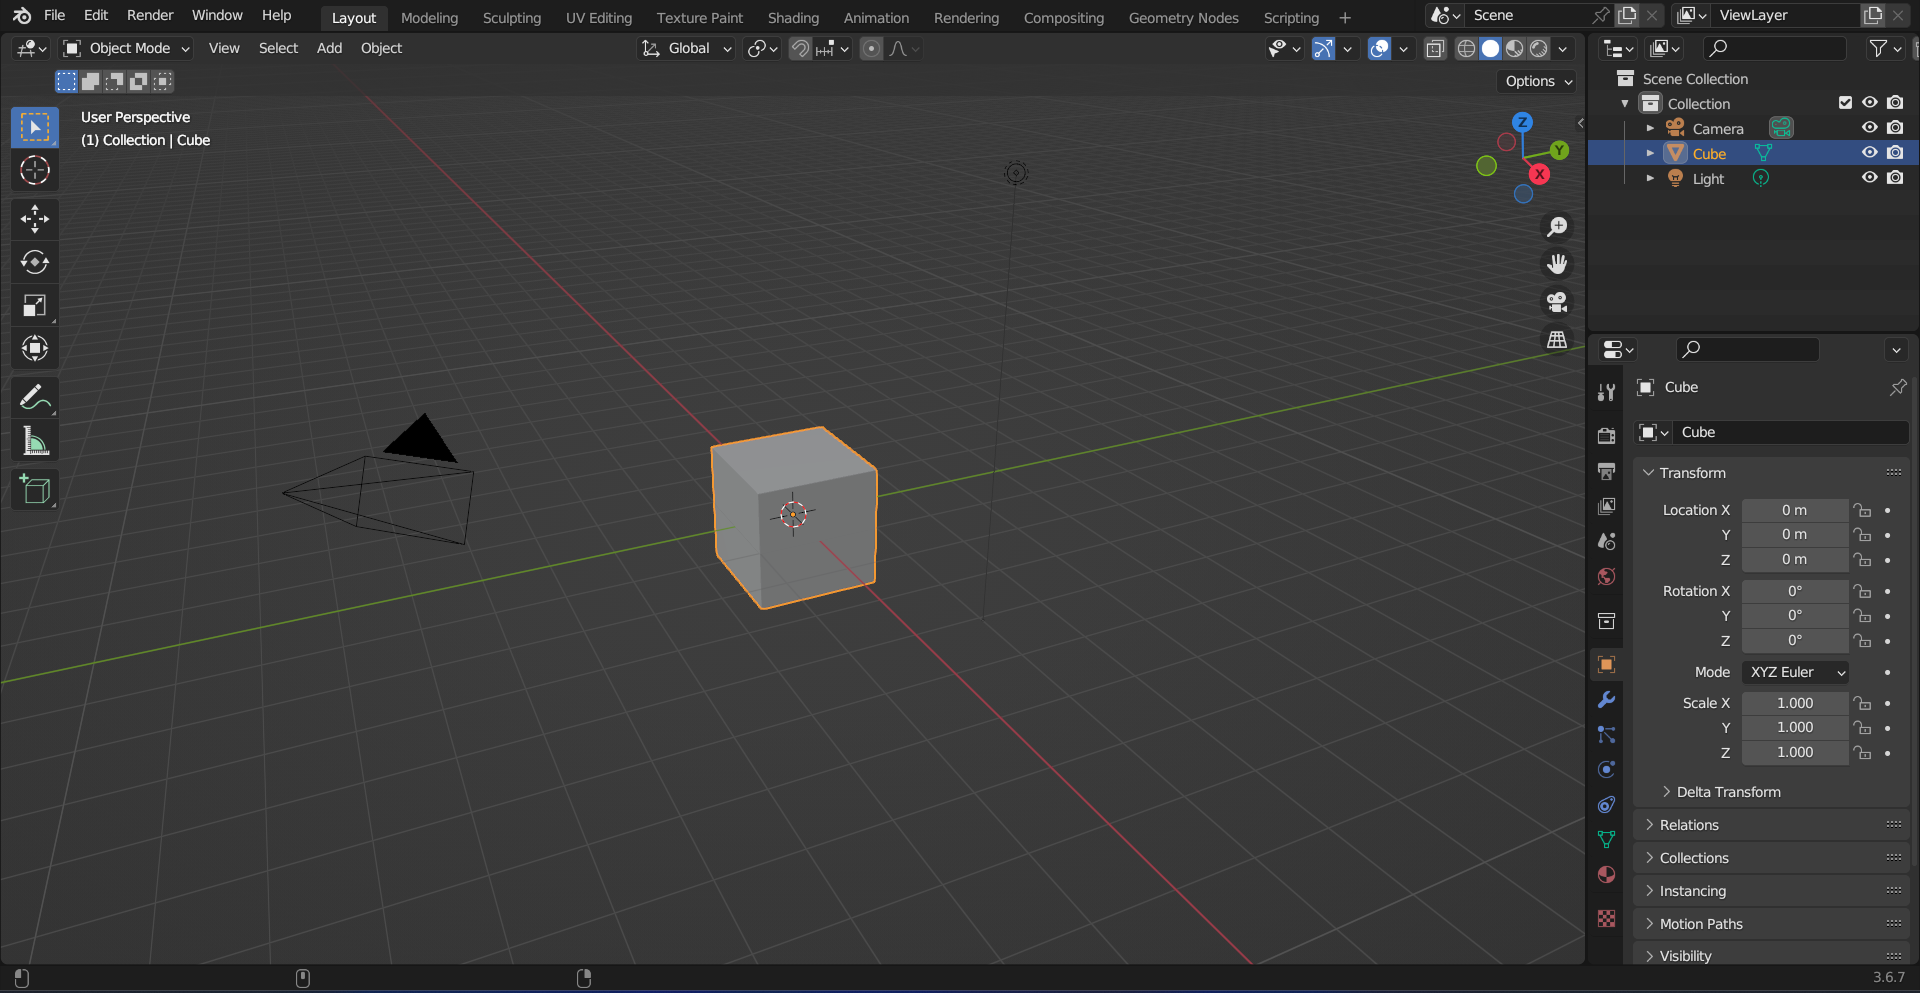
\includegraphics[width=1\textwidth]{images/defaultobjectmode.png}
\caption{Standard Ansicht im Object Mode}
\label{fig:defaultobjectmode}
\end{figure}

\item \textbf{Edit Mode:} Ist ein Modus für das Editieren einer Objektform mit verschiedensten Werkzeugen. Man kann die
einzelnen Vertices \footnote{Blender \cite{Vertices}}, Kanten und Flächen auf Basis von verschiedenen Kontrollpunkten bearbeiten.
\begin{figure}[h]
\centering
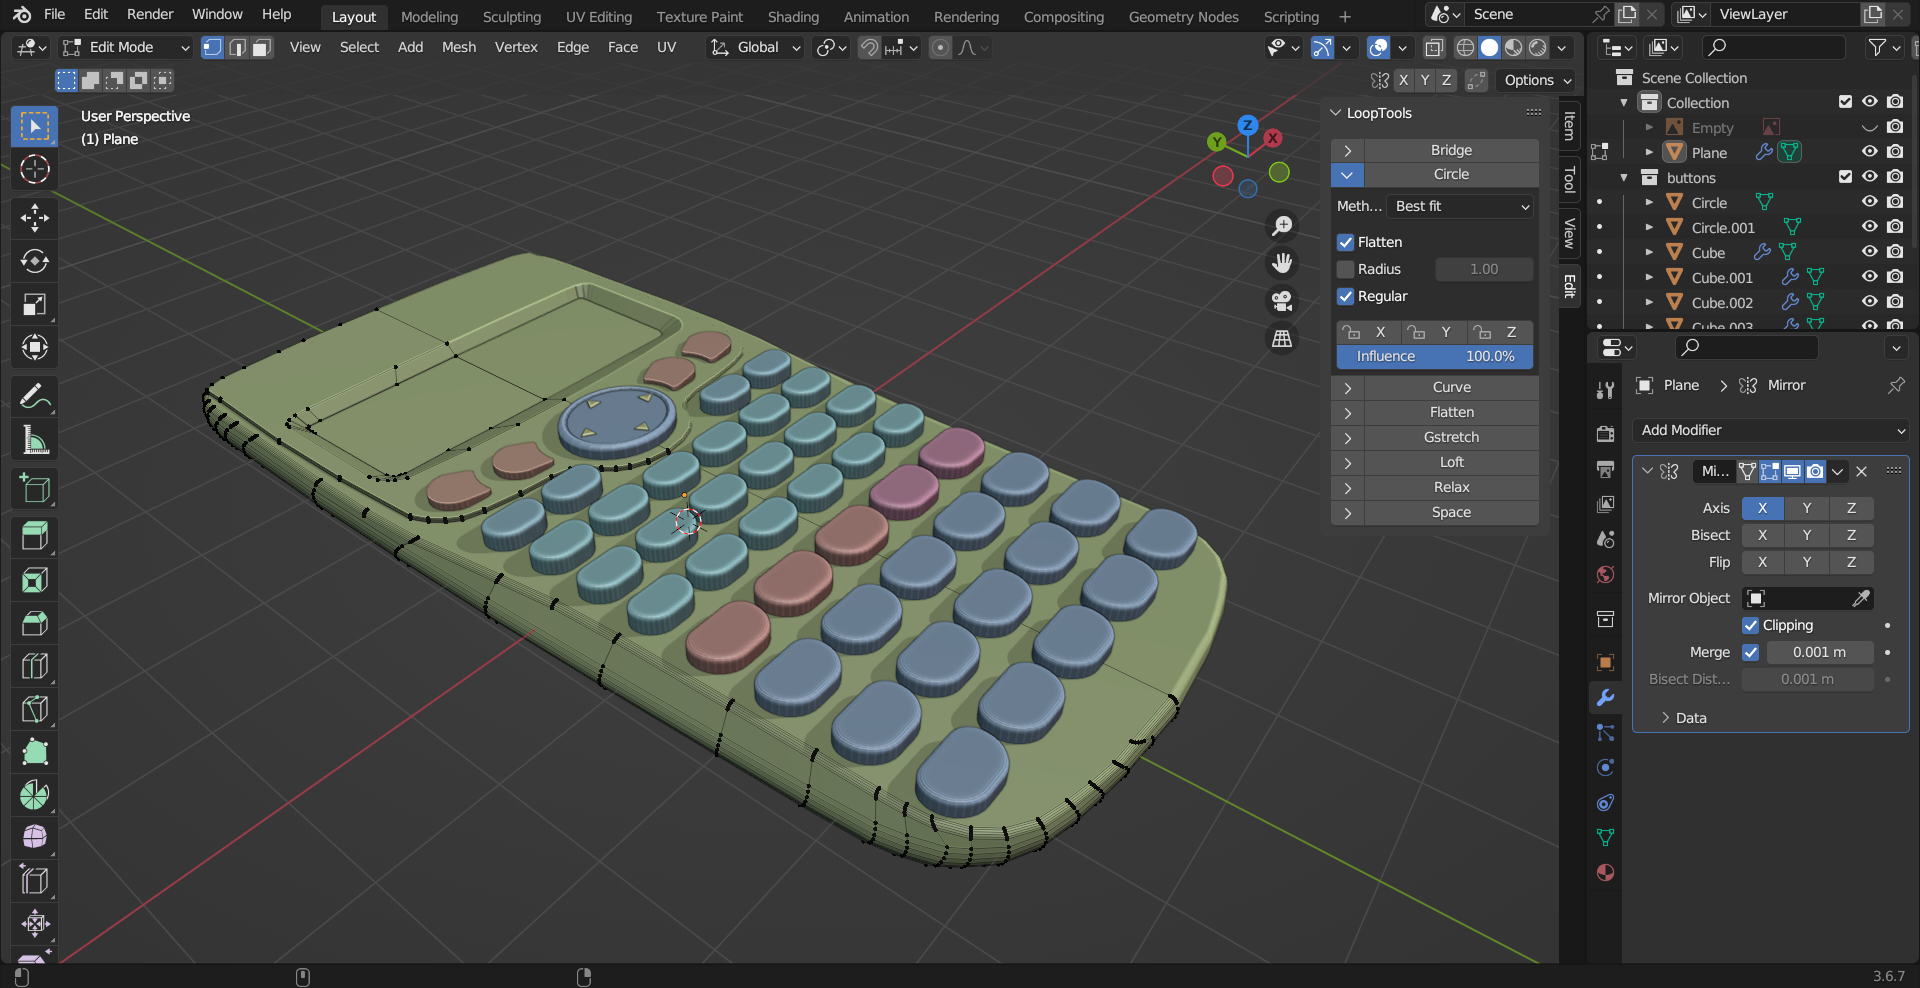
\includegraphics[width=1\textwidth]{images/calculatoreditmode.png}
\caption{Edit Mode Ansicht auf das Calculator Objekt}
\label{fig:calculatoreditmode}
\end{figure}

\item \textbf{Texture Paint Mode:} Ein Mesh-Only \footnote{Blender \cite{Mesh}} Modus der es dir ermöglicht Texturen direkt auf das Model im 3D-Viewport
zu zeichnen.
\begin{figure}[h]
\centering
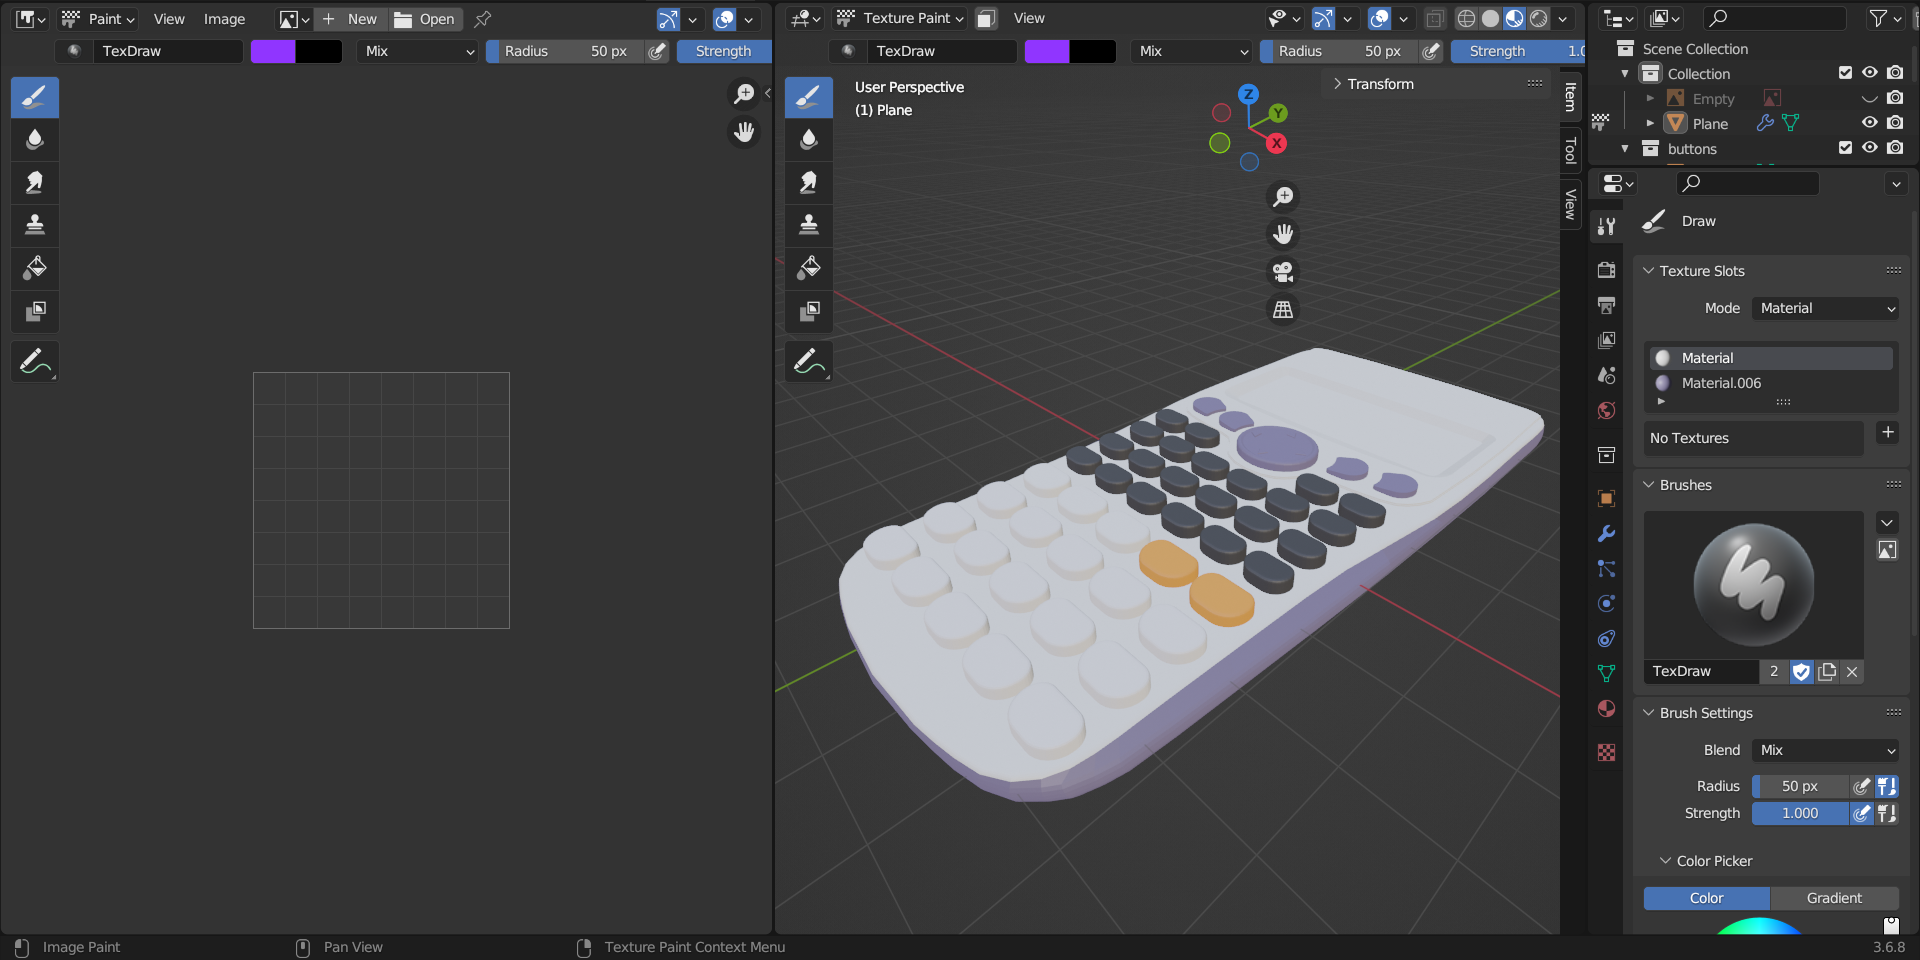
\includegraphics[width=1\textwidth]{images/texturepaintmode.png}
\caption{Standard Ansicht im Texture Paint Mode}
\label{fig:texturepaintmode}
\end{figure}
\end{itemize}

\subsection{Blender - Hierarchie}
Im folgenden Abschnitt wird erklärt, wie Blender aufgebaut ist und wie die einzelnen verwendeten Werkzeuge und Modifier
\footnote{Blender \cite{Modifier}} funktionieren. Es wurden einige Modelle erstellt, aber für ein einfacheres Verständnis
wurde für alle Beispielbilder das Taschenrechner-Modell verwendet.
\begin{figure}[h]
\centering
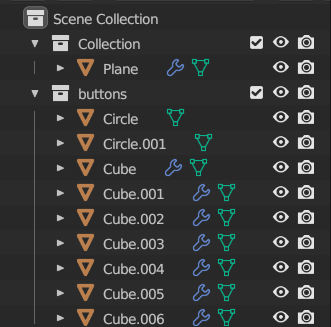
\includegraphics[width=0.8\textwidth]{images/blenderhierarchy.png}
\caption{Ansicht auf die Hierarchie des Taschenrechner Modells}
\label{fig:blenderhierarchy}
\end{figure}

In dieser Abbildung ist die Hierarchie und der Inhalt des Hauptmenüs zu sehen. Wie zu sehen ist, besteht die Szene aus
vielen wichtigen Komponenten die zusammenspielen, um die gewünschte Funktion zu erzielen. Darunter sind folgende Objekte:

\begin{itemize}
\item \textbf{Scene Collection:} Die umfassende Collection enthält das gesamte Modell mit allen Teilen. Collections
werden mehrmals in der Abbildung verwendet, um die Hierarchie besser zu strukturieren. Sie haben jedoch keinen Einfluss
auf das Objekt selbst.
\item \textbf{Plane:} Das Mesh dient zur groben Formgebung des Taschenrechners.
\item \textbf{Circles/Cubes:} Die Circles und Cubes sind die einzelnen Buttons.
\end{itemize}

In der Abbildung ist zu erkennen, dass einige Formen mit einem blauen/grünen Zeichen markiert sind.
Das blaue Zeichen kennzeichnet einen Modifier, das heißt, das Objekt hat einen oder mehrere Modifier.
Das grüne Zeichen steht für Data Properties und zeigt an, dass sich diese verändert haben.

\subsubsection{Blender - Modifier}
Im vorherigen Abschnitt wurden erwähnt das Modifier verwendet werden. Modifier ermöglichen verschiedene zusätzliche
Funktionen an einem Objekt.

\begin{figure}[h]
\centering
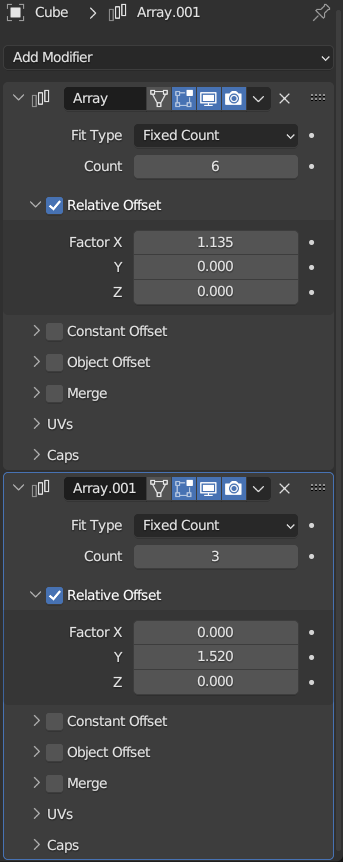
\includegraphics[width=0.8\textwidth]{images/blendermodifier.png}
\caption{Darstellung des benutzen Modifier im Taschenrechnermodell}
\label{fig:blendermodifier}
\end{figure}

In der Abbildung ist der Array Modifier zweimal zu sehen. Dieser wurde verwendet, um nicht jeden Knopf des Taschenrechners
einzeln modellieren zu müssen, sondern nur einen bestimmten Knopf horizontal oder vertikal mit beliebiger Versetzung zu
kopieren. Dabei haben die einzelnen Zeilen verschiedene Funktionen.
\begin{itemize}
\item \textbf{Fit Type:} Es besteht die Möglichkeit, entweder eine feste Anzahl von Objektkopien auszuwählen oder eine
Länge anzugeben, die dem Array entspricht.
\item \textbf{Count:} In dem Feld rechts daneben steht die Anzahl, wie oft das Objekt kopiert werden soll.
\item \textbf{Relative Offset:} Die relative Verschiebung basiert immer auf dem zuvor kopierten Modell und hat drei
Faktoren, die jeweils eine der drei Koordinaten darstellen. In diesem Fall soll es um 1.520 auf der x-Achse nach rechts
verschoben werden.
\end{itemize}

\section{Menü}
Im folgenden Abschnitt wird erläutert, wie das Menü in Unity hierarchisch aufgebaut ist und welche Schritte bis zur
endgültigen Version durchlaufen wurden.

\subsection{Version 1}
Ursprünglich war geplant, das UI/UX System mit einem Nahmenü zu implementieren, das dem Benutzer folgt und aus drei
Hauptbuttons und einem Pin-Button besteht. Der einfache Menüblock, der in Hüfthöhe schwebt, hat eine gewisse
innovative/neuartige Wirkung auf den Benutzer.

\begin{figure}[h]
    \centering
    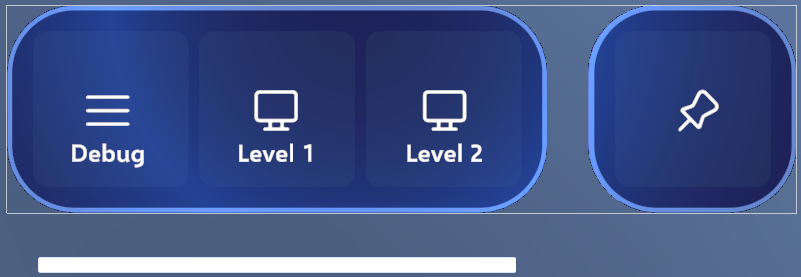
\includegraphics[width=0.8\textwidth]{images/menubar.png}
    \caption{Darstellung des Hauptmenüs im Unity Editor}
    \label{fig:menübar}
\end{figure}

\begin{figure}[h]
    \centering
    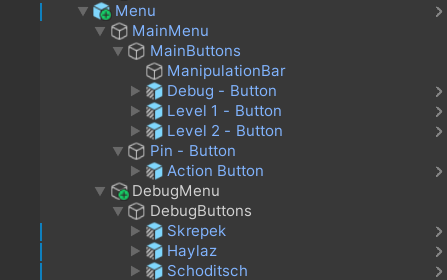
\includegraphics[width=0.8\textwidth]{images/menuHierarchy.png}
    \caption{Hauptmenühierarchie im Unity Editor}
    \label{fig:menühierarchy}
\end{figure}


In dieser Abbildung ist die Hierarchie und der Inhalt des Hauptmenüs zu sehen. Wie zu sehen ist, besteht die Szene aus
vielen wichtigen Komponenten die zusammenspielen, um die gewünschte Funktion zu erzielen. Darunter sind folgende Objekte:

\begin{itemize}
    \item \textbf{Menü:} Das Prefab, dem alle einzenen Buttons etc. zugewiesen sind.
    \item \textbf{ManipulationBar:} Ist ein GameObject, dem das \textit{ObjectManipulator.cs} Skript zugewiesen ist, welches
    die händische Menüführung ermöglicht.
    \item \textbf{Debug-Button:} Der Debug-Button ist ausschließlich für das Entwicklerteam vorgesehen. Beim Aktivieren öffnet
    sich ein erweitertes Menü oberhalb des Hauptmenüs, das zusätzliche Funktionen für das Bugfixing während des Betriebs
    bereitstellt.
    \begin{figure}[h]
        \centering
        
\includegraphics[width=0.8\textwidth]{images/debugmenubar.png}
        \caption{Darstellung des Debug Menüs im Unity Editor}
        \label{fig:debugmenübar}
    \end{figure}
    \item \textbf{Skrepek:} Das Prefab ist ein Button der für Skrepek vorbereitet ist, um mögliche Skripts für Bugfixing
    während des Betriebes einzubringen.
    \item \textbf{Haylaz:} Das Prefab ist ein Button der für Haylaz vorbereitet ist, um mögliche Skripts für Bugfixing
    während des Betriebes einzubringen.
    \item \textbf{Schoditsch:} Das Prefab ist ein Button der für Schoditsch vorbereitet ist, um mögliche Skripts für Bugfixing
    während des Betriebes einzubringen.
    \item \textbf{Level 1/2-Button:} Diese Prefabs stellen die Buttons für das Level wechseln da, ihnen ist das
    \textit{SceneChange.cs} Skript zugewiesen.
    \item \textbf{Pin-Button:} Der Pin-Button ermöglicht das Fixieren des Menüs an einer geeigneten Stelle. Dies ist besonders nützlich,
    wenn der Benutzer sich an einen Tisch setzt und das Menü entsprechend positionieren möchte. Die
    Positionierung erfolgt mithilfe der ManipulationsBar.
\end{itemize}

\subsubsection{Probleme bei Version 1}
Am Anfang war das Ziel, das Menü so einfach wie möglich zu gestalten. Trotzdem sollten alle notwendigen Funktionen integriert werden.
Nach mehreren Durchläufen und Tests mit projektunabhängigen Personen haben wir jedoch festgestellt, dass das ursprüngliche
Ziel ein großes Problem hat, es fehlt eine Dokumentation/Übersicht/Erklärung der Level. Als Benutzer wird man einfach ins
Hauptmenü geworfen, wo man nicht mehr sieht als die zwei klickbaren Levelbuttons.

\subsection{Version 2} %TODO: abbildung einfügen
Die Lösung für das vorherige Problem der fehlenden Übersicht ist das neue Menü. Dabei hat man sich an den derzeit
populären und trendigen AR/VR-Spielen orientiert und analysiert, warum die Benutzererfahrung dort deutlich besser ist
als in der vorherigen Version. Das Design wurde komplett überarbeitet, und das Nahmenü wurde entfernt. Stattdessen sind
im Hauptmenü, also dem Ladebildschirm, vormodellierte Objekte importiert, die mit Blender erstellt wurden und mit denen
der Nutzer interagieren kann. Diese Objekte, wie in der Abbildung ersichtlich, bestehen aus zwei Tafeln, die von unserem
Diplomarbeitslogo getrennt sind. Jede Tafel ist mit einem Text und einem dazugehörigen Titel des Levels ausgestattet.
Darunter befindet sich der Startbutton, der ebenfalls in Blender vormodelliert wurde. In Unity wurde ein unsichtbarer,
aber klickbarer Button mit genau denselben Maßen an die Stelle des Startbuttons eingefügt. An diesen Button ist das
\textit{SceneChange.cs}-Skript angehängt, welches im nächsten Punkt näher beschrieben wird.

Wenn ein Level in Version 2 geladen wird, gibt es im Gegensatz zu Version 1 ein anderes Menü. Das Ziel war es, die volle
Aufmerksamkeit des Benutzers auf das Level und die dortige Tätigkeit zu lenken. Daher wurde entschieden, auch das Nahmenü
aus den Leveln zu entfernen und stattdessen ein simples Handmenü einzubauen. Dieses Menü beinhaltet lediglich einen
Zurückknopf für das Hauptmenü. Die Idee hinter diesem Handmenü ist, dass es nur sichtbar ist, wenn der Benutzer es benötigt.
Das bedeutet, dass das Menü, also in diesem Fall nur der Zurückknopf, erst dann sichtbar wird, wenn der Benutzer seine
linke Hand umdreht und auf die Handfläche schaut.


\subsection{Laden der Level}
Der Button der im vorherigen Abschnitt bereits genannt wurde, wird im folgende Punkt näher beschrieben. Wenn man auf einen
beiden Start Knöpfe drückt, dann wird das Skript \textit{SceneChange.cs} ausgeführt. Dieser Code ist für die Änderung auf
eine andere/neue Szene verantwortlich. Die zu ladende Szene wird dabei in Unity Inspector selbst festgelegt, der Code greift
dann auf die Variable mit den jeweiligen Szenennamen zu. Bei dem linken Knopf ist es die Szene \textit{Level1} und bei dem
rechten Knopf ist es die Szene \textit{Level2}.

\begin{lstlisting}[style=csharp, caption=Auf Knopfdruck Szene wechseln. label=code:scenechange]
using UnityEngine;
using UnityEngine.SceneManagement;

public class SceneChanger : MonoBehaviour
{
    public string sceneToLoad;

    public void ChangeScene()
    {
        if(SceneManager.GetActiveScene().name != sceneToLoad)
        {
            PlayerPrefs.DeleteAll();
            SceneManager.LoadScene(sceneToLoad, LoadSceneMode.Single);
        }
    }
}
\end{lstlisting}

Die Hauptkomponenten des Codes sind:
\begin{itemize}
\item{sceneToLoad:} Dies ist eine öffentliche Variable vom Typ String, die den Namen der zu ladenden Szene enthält. Sie
kann im Unity-Inspector definiert werden, um die Zielszene anzugeben (siehe Zeile 6).
\item{ChangeScene():} Dies ist eine öffentliche Methode, die aufgerufen wird, um die Szene zu wechseln. Sie prüft dass
die aktive Szene nicht mit der in \textit{sceneToLoad} angegebenen Szene identisch ist.
\item{SceneManager.GetActiveScene().name:} Dies ruft den Namen der aktuell geladenen Szene ab.
\item{PlayerPrefs.DeleteAll():} Diese Methode löscht alle gespeicherten PlayerPrefabs, was hilfreich sein kann, um
sicherzustellen, dass keine alten Daten zwischen den Szenenwechseln erhalten bleiben (siehe Zeile 12). Ist vor allem wichtig,
da wir ohne das Löschen der PlayerPrefabs Probleme mit dem HoloLens Cache beim Wechseln innerhalb der Szenen hatten.
\item{SceneManager.LoadScene(sceneToLoad, LoadSceneMode.Single):} Diese Methode lädt die in \textit{sceneToLoad}
gespeicherte Szene im Single-Modus, d.h. die aktuelle Szene wird entladen und die neue Szene geladen (siehe Zeile 13).
\end{itemize}

%idk
\begin{figure}[h]
\centering
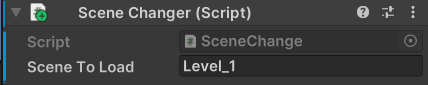
\includegraphics[width=0.8\textwidth]{images/sceneToLoad.png}
\caption{Darstellung der SceneToLoad Variable, anhand des Level_1 Buttons.}
\label{fig:scenetoload}
\end{figure}

\subsection{Setzen des Menüs}
Da sich das alte Menü in Version 1 automatisch mit dem Benutzer bewegte, war es kein Problem, es in das Hauptmenü zu laden,
aber bei den neuen Modellen in Version 2 muss man das Menü selbst platzieren. Dafür gibt es das Skript \textit{MenuSpawn.cs}.

\begin{lstlisting}[style=csharp, caption=Auf Knopfdruck Szene wechseln. label=code:spawnmenu]
using System.Collections;
using System.Collections.Generic;
using UnityEngine;

public class SpawnPrefab : MonoBehaviour
{
    public GameObject menu;

    void Start()
    {
        SpawnPrefabMenu();
    }

    void SpawnPrefabMenu()
    {
        Vector3 cameraPosition = Camera.main.transform.position;
        Vector3 spawnPosition = new Vector3(cameraPosition.x, cameraPosition.y, cameraPosition.z + 1f);
        Instantiate(menu, spawnPosition, Quaternion.identity);
        menu.SetActive(true);
    }
}
\end{lstlisting}

Beim Start der Anwendung wird die Methode \textit{SpawnPrefabMenu()} ausgeführt. Diese Methode ist für die Positionierung
des Menüs verantwortlich. Die im Codeabschnitt \ref{code:spawnmenu} ersichtlichen Positionsvektoren sind einerseits dafür
zuständig, die aktuelle Kameraposition zu ermitteln, aber auch eine neue Spawnposition zu setzen, die um 1 auf der z-Achse
versetzt ist, so dass das Menü vor dem Benutzer erscheint. Der \textit{Instantiate} ist dafür verantwortlich, dass das Menü
an der jeweiligen Spawnposition gesetzt wird. Anschließend wird das zuvor versteckte Menü mit \textit{menu.SetActive(true)}
aktiviert, so dass der Benutzer es sehen und mit ihm interagieren kann.

\subsection{UI/UX}
Im folgenden Abschnitt werden die Ziele genannt, auf die sich bei der Menüerstellung konzentriert wurde.
\begin{itemize}
\item \textbf{Blickzentrierung und Interaktionsmodelle:}
Die Menüleiste bewegt sich auf Hüfthöhe mit dem Benutzer mit und ermöglicht so eine natürliche und intuitive Interaktion.
Der Benutzer kann die Bedienelemente einfach durch Blickkontakt auswählen, was die Benutzerfreundlichkeit erhöht und die
Bedienung der Anwendung erleichtert.
\item \textbf{Konsistenz im Design:}
Die klare Gestaltung der Buttons mit aussagekräftigen Symbolen trägt zur Konsistenz und Benutzerfreundlichkeit bei.
Eine einheitliche visuelle Sprache erleichtert es dem Benutzer, die Funktionen der Buttons zu verstehen, selbst wenn er
sie zum ersten Mal verwendet.
\item \textbf{Kontextsensitive Funktionen:}
Der Debug-Button bietet erweiterte Funktionen, die speziell für Entwickler relevant sind. Diese kontextsensitiven
Optionen sind wichtig für die Fehlersuche und tragen dazu bei, die Entwicklungszeit zu optimieren. Gleichzeitig bleibt
die Benutzeroberfläche für den Endbenutzer sauber und übersichtlich.
\item \textbf{Anpassungsmöglichkeiten für den Benutzer:}
Die Option, das Menü mit dem Pin-Button zu fixieren und mit der Grab-Bar frei zu bewegen, gibt dem Benutzer die
Kontrolle über die Positionierung des Menüs. Diese Anpassungsmöglichkeiten tragen dazu bei, die Anwendung an
verschiedene Nutzerszenarien anzupassen und die individuellen Bedürfnisse der Benutzer zu berücksichtigen.
Feedback und Animationen
\end{itemize}

\section{Ping Level}
In diesem Level wird das IT-Grundprinzip eines Pings zwischen zweier
PCs dargestellt. Das Kabel zwischen den zwei PCs wird von der
HoloLens getracked und mittels Kurvenberechnung wird dann eine
unsichtbare Kurve über dieses Kabel gezeichnet. Wenn dann der Benutzer
auf die Enter Taste auf einem PC drückt wird ein Ping-Paket simuliert
und auf dieser Kurve von einem PC zu dem anderen geschickt.

\subsection{Object Tracking}
Durch verwendung von bereitgestellten Technologien der HoloLens2
werden die zwei PCs und das Kabel getracked.
%Hier dann noch code zum Object Tracking einfügen

\subsection{Kurvenberechnung}
Durch Berechnung der Kurve wird das Kabel als Kurve gespeichert
und dadurch wird es ermöglicht, dass das 3D-Ping-Paket über diese
Kurve von einem PC zum anderen läuft.
%Hier dann noch code zur Kurvenberechnung einfügen

\section{Knapsack Problem Level}
Im zweiten Level dieses Projekts steht das Knapsack-Problem im Fokus.
Ziel ist es, diesen Programmieralgorithmus mithilfe von Augmented Reality
(AR) visuell darzustellen. Dieser Algorithmus wird nicht nur in der Höheren
Technischen Lehranstalt (HTL) vermittelt, sondern die Benutzer sollen
ihn auch selbst programmieren können.

Der Level beginnt damit, dass der Benutzer aufgefordert wird, auf eine
horizontale, flache Oberfläche zu schauen. Diese Oberfläche kann ein Tisch,
der Boden oder ähnliches sein. Der Benutzer wird dann gebeten, für eine bestimmte
vorgegebene Zeit auf diese Oberfläche zu schauen. Nach Ablauf der vorgeschriebenen
Zeit wird dann das Inventar als auch das \textit{infoObjekt} platziert.

Das Inventar wird durch ein 3x3 zweidimensionales Gitter repräsentiert, ähnlich
wie das Inventar in einem Spiel. Zusätzlich befinden sich auf der Oberfläche 11 Bauklötze,
die mit QR-Codes versehen sind. Diese Bauklötze repräsentieren die Items, die der Benutzer
in das Inventar legen kann. Durch Aufheben und Nahheranhalten an die HoloLens wird der QR-Code gescannt.
Dadurch werden das dazugehörige 3D-Modell, der Wert, Gewicht und der Name des Items angezeigt.
Diese Informationen sind für den Benutzer wichtig, um das Gewicht des Items und
seinen Einfluss auf das Inventar zu verstehen.

Wenn der Bauklotz erfolgreich platziert wurde, wird automatisch der Knapsack-Algorithmus für die perfekte Lösung,
und die Berechnung des eigenen Inventars gestartet um stets den aktuellen Wert zu sehen.

Insgesamt bietet dieses Unity Level für die HoloLens 2 eine interaktive und visuelle Erfahrung,
bei der die Benutzer das Knapsack-Problem nicht nur verstehen, sondern auch praktisch anwenden können.

\subsection{Knapsack-Problem Level Hirarchie}
In dem folgendem Abschnitt wird darauf eingegangen wie eine Szene in dem Unity Editor aufgebaut ist und wie diese Grundsätzlich
funktionieren.\\

\begin{figure}[h]
    \centering
    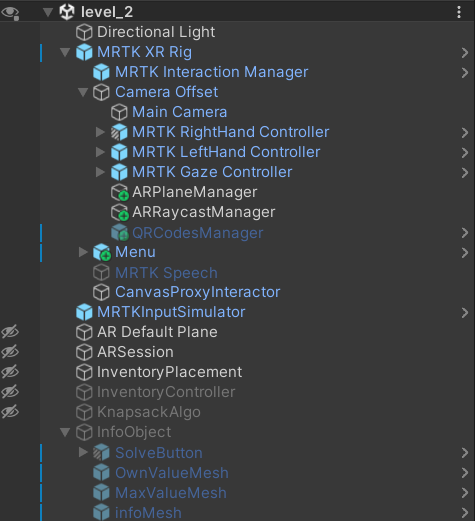
\includegraphics[scale=0.8]{images/Level2Hirarchy}
    \caption{Knapsack-Problem Levels Hirarchie Unity Editor.}
    \label{fig:level2_hierarchy}
\end{figure}

In dieser Abbildung ist die Hirarchie und der Inhalt des Knapsack-Problem Levels / Szene-2\footnote{Unity \cite{Scene}} zu sehen.
Wie zu sehen ist, besteht die Szene aus vielen wichtigen Komponenten die zusammenspielen, um das gewünschte Ergebnis
zu erzielen. Darunter sind folgende Objekte:

\begin{itemize}
    \item \textbf{level-2}\\
    Die Scene in der Alle Unity-Game-Objekte enthalten sind.
    \item \textbf{AR Default Plane}\\
    In der Augmented Reality (AR)-Entwicklung bezieht sich ein Plane\footnote{Unity \cite{Plane}} normalerweise
    auf eine erkannte horizontale Fläche in der realen Welt, auf der virtuelle Objekte platziert werden können. Diese
    Flächen können zum Beispiel Tische, Böden oder andere ebene Oberflächen sein. Das Erkennen und Tracking von Planes
    ist entscheidend, um AR-Objekte realistisch in die Umgebung zu integrieren.
    \item \textbf{ARSession}\\
    In Unity und AR Foundation bezieht sich die ARSession im Allgemeinen auf die Hauptkomponente, die die AR-Funktionalitäten
    steuert und koordiniert.
    \item \textbf{InventoryPlacementController}\\
    Ist ein Game Objekt, dem das \textit{InventoryPlacementController.cs} Script zugewiesen ist und
    bei Szenen-Start aktiv ist. Dieses Game Objekt kümmert sich darum, dass das Inventar richtig in der Augmented Reality
    Welt platziert wird.
    \item \textbf{InventoryController}\\
    Das Game Objekt, dem das \textit{InventorryController.cs} Script zugewiesen ist und nach Abschluss des InventoryPlacement
    Scripts aktiviert wird. Dieses Objekt ist die Hauptschnittstelle zwischen den QR-Codes und dem 3D Inventar Modell und
    kümmert sich darum neue QR-Codes innerhalb des Modells zu erkennen und zu verspeichern.
    \item \textbf{KnapsackSolver}\\
    GameObjekt, dem das \textit{KnapsackSolver.cs} Script zugewiesen ist und bei platzieren eines QR-Codes innerhalb des
    Inventars auslöst, den maximalen erreichbaren Wert, die perfekte Lösung und den Wert des selbst erstellten Inventars
    berechnet.
    \item \textbf{bestSolutionPrefab}\\
    Dieses Objekt ist das Prefab\footnote{Unity \cite{Prefab}} für die Perfekte Lösung. Diesem Objekt ist das 3D Modell
    des Inventars untergeordnet und diesem Inventar sind Prefabs für QRCodes untergeordnet. In jeder Zelle des Inventars
    ist ein eigenes QRCode Prefab um anschließend die berechnete perfekte Lösung darstellen zu können. Diesem Objekt ist
    das \textit{PerfectSolutionVisualizer.cs} Script zugewiesen, dass sich darum kümmert die perfekte Lösung anzuzeigen.
    \item \textbf{InfoObject}\\
    Dieses Game Objekt ist eine Sammlung aus mehreren Unity Game Objekten. Dieses Objekt wird bei platzieren
    des Inventars neben dem Inventar mitplatziert. Bei den Objekten handelt es sich hierbei um den \textit{BestSolutionButton},
    der bei Knopfdruck einer der mehreren besten Lösungen visuell veranschaulicht, und drei \textit{TextMeshes}, um die
    berechneten Werte, und auch Informationen anzuzeigen. Zusätzlich ist hier zusehen, dass diese 4 Objekte dem \textit{infoObject}
    untergeordnet sind, was bedeutet, dass diese Objekte\textit{children} von dem \textit{infoObejct} sind. Das übergeordnete
    Objekt wird hier dann als \textit{parent} bezeichnet.
\end{itemize}

In der Abbildung ist zu sehen, dass ein Paar Game Objekte ausgegraut und nicht ausgegraut sind und, dass neben ein paar Game Objekten ein durchgestrichenes Auge zu sehen ist.
Wenn ein Game Objekt im Unity Editor ausgegraut ist bedeutet das, dass dieses GameObjekt und somit alle angehängiten Scripts von diesem Game Objekt deaktiviert sind.
Das bedeutet, dass dieses Game Objekt samt allen Scripts zu Szenenbeginn nicht aufgerufen und somit auch nicht ausgeführt werden. Nicht ausgegraute Game Objekte widerum sind
daher genau das Gegenteil. Das beudetet, dass das Game Objekt selbst samt allen angehängiten Scripts alle aktiviert sind und somit zu Szenenbeginn aufgerufen und ausgeführt werden.

Wenn neben einem Game Objekt das durchgestrichene Auge zu sehen ist bedeutet das nur, dass dieses Game Objekt im Unity Editor nicht zu sehen ist. Andererseits, wenn kein Zeichen
neben dem Game Objekt zu sehen ist, ist dieses Objekt im Unity Editor sichtbar. Dies dient dazu, dass falls in der Unity Szene viele Game Objekte vorhanden sind, dass man
diejenige ausblendet die nicht im Editor sichtbar sein müssen wie zum Beispiel Tesh Meshes oder Lables.

\subsection{Nutzung von QR-Codes}
Im vorherigen Abschnitt wurde bereits erwähnt, dass QR-Codes in diesem Level verwendet werden, um verschiedene Elemente
zu repräsentieren. Diese QR-Codes spielen eine entscheidende Rolle, indem sie dazu dienen, vielfältige Informationen zu
den einzelnen Objekten zu speichern und sie anschließend in einer virtuellen Umgebung abzubilden. Im folgenden Abschnitt
möchten wir näher darauf eingehen, wie genau diese QR-Codes generiert werden und welchen Zweck sie innerhalb der
Augmented Reality (AR)-Applikation erfüllen. Dabei wird insbesondere betrachtet, wie die Generierung der Codes erfolgt
und auf welche Weise sie innerhalb der Anwendung zur Interaktion mit den realen Objekten verwendet werden.

\subsubsection{Struktur und Inhalt eines QR-Codes}
Die Informationen, die in einem QR-Code gespeichert werden können, sind begrenzt. In unserem Anwendungsfall wird lediglich
eine einzelne Zahl im Bereich von 1 bis 11 abgespeichert. Diese Zahlen repräsentieren die 11 verschiedenen Modelle, die
wir unterscheiden möchten. Da nur eine Zahl gespeichert wird, genügt ein QR-Code der Größe 21x21 Module (Version 1). Die
geringe Anzahl von Modulen ermöglicht eine schnellere Erkennung, auch über größere Distanzen.
%TODO: Testen und Grafik erstellen um zu zeigen das es eine Rolle spielt welche version wir verwenden + wie groß die sind

Die zugehörigen Zahlen erhalten in der Software, genauer gesagt in der Klasse \textit{QRItem.cs}, einen Kontext. Der folgende Codeausschnitt zeigt dies:

\begin{lstlisting}[style=csharp, caption={}, label=code:update]
public class QRItem
{
    public struct QRData
    {
        public int id;
        public string name;
        public Vector3 position;
        public int weight;
        public int value;
    }

    public QRData qrData;

    public Dictionary<int, QRData> items = new Dictionary<int, QRData>()
    {
        {1, new QRData { id = 1, name = "Laptop", weight = 70, value = 100 }},
        {2, new QRData { id = 2, name = "Router", weight = 25, value = 50 }},
        {3, new QRData { id = 3, name = "Maus", weight = 20, value = 30 }},
        // ...
        {11, new QRData { id = 11, name = "Handy", weight = 30, value = 100 }}
    };

    public QRItem(int id)
    {
        items.TryGetValue(id, out qrData);
    }
}
\end{lstlisting}

In dieser Klasse wird ein Dictionary verwendet, das den Zahlen die folgenden Informationen zuordnet:

\begin{itemize}
    \item \textbf{Item Id:} Die numerische Kennung im QR-Code.
    \item \textbf{Item Name:} Die Bezeichnung des Items, das dieser QR-Code repräsentiert.
    \item \textbf{Item Position:} Die Position des Items in der virtuellen Umgebung.
    \item \textbf{Item Weight:} Das Gewicht des Items.
    \item \textbf{Item Value:} Der Wert des Items.
\end{itemize}

Diese Informationen spielen eine wesentliche Rolle in der weiteren Berechnung des Knapsack-Algorithmus.

\subsubsection{QR-Code-Tracking}
Das Tracking der QR-Codes erfolgt mithilfe des \textit{QRCodeManager.cs} Skripts. Dieses Klasse ist ein Singleton, das
die Erkennung und Verfolgung der QR-Codes steuert.

Nach der Erkennung eines QR-Codes erfolgen eine Reihe von Schritten, um diese Informationen zu speichern, verarbeiten
und zuletzt darzustellen.
Hier eine kurze Übersicht:
%TODO: Übersicht einfügen
\begin{itemize}

\item \textbf{Initialisierung des QR-Tracking-Systems:}
Zur Aktivierung des QR-Tracking-Systems werden die erforderlichen Ressourcen und Komponenten gestartet, um die Erkennung
von QR-Codes zu ermöglichen. Dabei werden Tracking-Algorithmen gestartet, die für die Lokalisierung und Identifizierung
von QR-Codes in der Umgebung benötigt werden. Diese Initialisierung erfolgt zu Beginn der Anwendungsaktivität.

\item \textbf{Zugriffsanforderung auf die Kamera der Brille:}
%TODO: Hier Bild von "Camera acess needed" einfügen
Für das QR-Tracking wird der Zugriff auf die Kamera der Augmented-Reality-Brille benötigt. Eine Zugriffsanfrage wird
gestellt, um die notwendigen Berechtigungen zu erhalten. Dieser Schritt ist entscheidend, um visuelle Daten von der Kamera
zu erhalten und QR-Codes in der physischen Umgebung zu erkennen.

\item \textbf{Einrichtung des QR-Trackings:}
Die Einrichtung des QR-Trackings umfasst die Konfiguration von Parametern und Einstellungen, die für die korrekte
Funktion des Tracking-Systems erforderlich sind.Dazu gehören Kalibrierungsschritte, die Anpassung an die Umgebung und die
Festlegung von Erkennungsbereichen. Eine ordnungsgemäße Einrichtung gewährleistet eine zuverlässige und präzise Erkennung von QR-Codes.

\item \textbf{Starten des QR-Trackings:}
Das System sucht aktiv nach QR-Codes in der Umgebung, um sie zu erkennen. Die Kamera erfasst kontinuierlich visuelle
Daten, welche von den Tracking-Algorithmen analysiert werden, um QR-Codes zu identifizieren. Das Starten des Trackings
markiert den Beginn des fortlaufenden Erkennungsprozesses.

\item \textbf{Erkennung eines QR-Codes (Event):}
Sobald die Kamera einen QR-Code erfasst, wird dieser erkannt. Das Ereignis signalisiert, dass ein QR-Code erkannt wurde
und gibt Informationen über den erkannten QR-Code, wie seine Daten und Position, weiter.

\item \textbf{Zuweisung des erkannten QR-Codes zum Objekt:}
Nach der Erkennung wird überprüft, ob der erkannte QR-Code bereits in der Anwendung registriert ist. Falls dies der Fall
ist, wird der erkannte QR-Code einem entsprechenden Objekt in der virtuellen Umgebung zugeordnet.

\item \textbf{Instanzierung des QRCode-Objekts:}
Anschließend wird ein Objekt instanziiert, das den erkannten QR-Code repräsentiert. Dieses Objekt wird oft als
QR-Objekt bezeichnet und enthält visuelle Darstellungen, Interaktionsmöglichkeiten und weitere Informationen über das
zugeordnete Objekt enthalten. Durch die Instanzierung kann der erkannte QR-Code in die virtuelle Umgebung integriert werden.

\item \textbf{Aktualisierung der Eigenschaftenanzeige:}
Die Aktualisierung der Eigenschaftsanzeige dient dazu, visuelle und informative Darstellungen des erkannten QR-Codes zu
aktualisieren. Hierbei werden die Position, Größe, visuelle Darstellung und zugehörige Informationen des QR-Codes aktualisiert.
Durch die Aktualisierung wird sichergestellt, dass die Benutzer stets die neuesten Informationen über das durch den QR-Code
repräsentierte Objekt erhalten.

\end{itemize}

\subsubsection{Interaktion mit QR-Codes}
%TODO: Bild einfügen von bauklötzen und QR-Codes
Durch die Verwendung der HoloLens können wir dem Benutzer eine visuelle Darstellung einer virtuellen Welt bieten. Um eine
Verbindung zwischen der realen und der virtuellen Welt herzustellen, nutzen wir QR-Codes.  Diese dienen als Repräsentationen
der realen Objekte, die wir in der virtuellen Welt darstellen möchten.

Wie in Abbildung 1 zu sehen ist, sind die Bauklötze mit QR-Codes versehen. Diese Bauklötze repräsentieren die Gegenstände,
die der Benutzer in sein Inventar aufnehmen kann. Wenn der Benutzer einen Bauklotz aufhebt und ihn der HoloLens nähert, wird
der QR-Code gescannt. Dadurch werden Informationen wie das zugehörige 3D-Modell, der Wert, das Gewicht und der Name des
Gegenstands angezeigt. Auf diese Weise können wir eine nahtlose Verbindung zwischen der realen und der virtuellen Welt
herstellen und dem Benutzer eine interaktive Erfahrung bieten.

Dem Benutzer wird die Möglichkeit geboten, die Bauklötze physisch zu berühren, aufzuheben und zu fühlen. Diese sensorische
Erfahrung trägt dazu bei, die Immersion des Benutzers zu verbessern und ihm ein besseres Verständnis der virtuellen Welt
zu ermöglichen.

\subsubsection{Bestimmen der Position QR-Codes}
%TODO: Auch die events add remove und update erklären vom qrWatcher

\subsubsection{Visualisierung von QR-Codes}
%TODO: Bild von einem QR Prefab einfügen

\subsubsection{Zugriff auf QR-Codes erteilen}

\subsection{Inventory Placement Controller Game Objekt}
Um eine präzise Interaktion zwischen der realen und augmentierten Realität zu gewährleisten, ist der Zugriff auf die Kamera
erforderlich, um die physische Umgebung präzise zu erfassen. Durch die Analyse der erfassten Umweltdaten können relevante
Ebenen identifiziert werden, die entscheidend sind, um eine akkurate Platzierung des Inventar-Objekts zu gewährleisten.

In diesem Abschnitt wird das \textit{Inventory Placement Controller} Game Objekt mit dem angehängten
\textit{InventoryPlacementController.cs} Script behandelt. Letzteres beinhaltet die \textbf{InventoryPlacementController}
Klasse, welche sämtliche Funktionen zur Berechnung und Platzierung des Inventars umfasst. Diese Funktionalitäten werden
im Folgenden detailliert erläutert.

\begin{figure}[h]
    \centering
    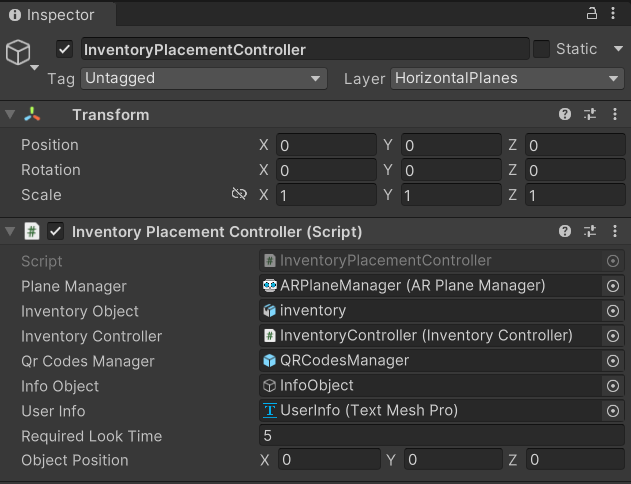
\includegraphics[scale=0.8]{images/invPlace_Editor}
    \caption{inventoryPlacement Objekt im Editor}
    \label{fig:inventoryPlacementController_Editor}
\end{figure}

Die Darstellung des \textit{inventoryPlacementController}-Objekts im Unity Editor, wie sie in
Abbildung \ref{fig:inventoryPlacementController_Editor} gezeigt wird, bietet eine Schnittstelle zur Konfiguration
verschiedener Parameter. Hierzu zählen insbesondere die Zuweisung der Ebenenposition, die Feinjustierung der Koordinaten
innerhalb des Unity Editors sowie die Verbindung mit der Komponente \textit{InventoryPlacementController.cs}. Zusätzlich
werden voreingestellte Werte für Schlüsselvariablen angezeigt, die für die Ausführung des Codes von entscheidender Bedeutung
sind. Diese Auflistung und Erläuterung dieser Variablen umfasst:

\begin{itemize}
    \item \textbf{Raycast Manager:} Diese Variable dient als Verweis auf das Game Objekt des \textit{ARRaycastManagers}
    aus der Szene Level 2.
    \item \textbf{Plane Manager:} Hierbei handelt es sich um eine Zuweisung zum Game Objekt des \textit{ARPlanesManagers}
    aus der Szene Level 2.
    \item \textbf{Inventory Object:} Diese Referenz ist mit dem 3D-Modell des Inventars aus dem Prefab-Ordner verknüpft.
    \item \textbf{Inventory Controller:} Diese Variable ist mit dem Skript des \textit{InventoryControllers} verbunden.
    \item \textbf{QR Codes Manager:} Hierbei handelt es sich um einen Verweis auf das Game Objekt des \textit{QRCodeManagers}
    aus der Szene Level 2.
    \item \textbf{Info Object:} Diese Referenz ist mit dem Game Objekt \textit{infoObject} aus der Szene Level 2 verbunden.
    \item \textbf{Required Look Time:} Diese Variable gibt die vorgeschriebene Zeitdauer an, für die der Benutzer auf ein
    Plane blicken muss, damit das Inventar platziert wird.
\end{itemize}

Durch den Unity Editor besteht die Möglichkeit, die Werte dieser Variablen direkt zu manipulieren, was direkte Auswirkungen
auf die Ausführung des Codes hat. Diese direkte Manipulation bietet eine intuitive und effiziente Möglichkeit, die
Einstellungen anzupassen und die Funktionalität des Programms entsprechend anzupassen.

\subsubsection{InventoryPlacementController Klassenvariablen}
\begin{lstlisting}[style=csharp, caption={Klassenvariablen der InventoryPlacementController Klasse}, label=code:anchor_var]
public ARRaycastManager raycastManager;
public ARPlaneManager planeManager;
public GameObject inventoryObject;
public InventoryController inventoryController;
public GameObject qrCodesManager;
public GameObject infoObject;
public float requiredLookTime = 5.0f;
public Vector3 objectPosition;

private ARPlane selectedDeskPlane;
private float lookStartTime = -1f;
private bool objectPlaced = false;
private float heightOffset = 0.001f;

private bool canStartScript = false;
\end{lstlisting}

Die dargestellten Klassenvariablen in Codeabschnitt \ref{code:anchor_var} sind integraler Bestandteil der
\textit{PlaceObjectOnLookedAtDesk}-Klasse. Öffentliche (\textbf{public}) Variablen repräsentieren Objekte und Werte, die
im Unity Editor festgelegt und übergeben werden können oder von anderen Klassen für die Funktionalität benötigt werden.
Dies ermöglicht einen direkten Zugriff auf diese Objekte sowohl innerhalb der eigenen Klasse als auch von anderen Klassen
aus. Die Vektor-Variable \textit{objectPosition} spielt dabei eine entscheidende Rolle für die präzise Platzierung der
Objekte.

Hingegen dienen die privaten (\textbf{private}) Variablen der lokalen Speicherung von Werten, die ausschließlich innerhalb
der Klasse benötigt werden und von keiner anderen Klasse verwendet werden sollen.

Dieser Ansatz der Kapselung von Daten erlaubt eine klare Trennung zwischen öffentlich zugänglichen Daten und internen
Variablen, was eine effiziente und strukturierte Entwicklung und Wartung des Codes ermöglicht.

\subsubsection{Startverzögerung}
\begin{lstlisting}[style=csharp, caption={Beginn des Inventory Placement Controllers}, label=code:Start]
void Start()
{
    StartCoroutine(DelayedStart());
}
\end{lstlisting}
Die Lebenszyklusmethode \textbf{Start()} wird zu Beginn des Levels für das "Knapsack-Problem" aufgerufen, wie im
Codeausschnitt \ref{code:Start} gezeigt. Diese Methode initiiert die Coroutine \textbf{DelayedStart()}, die eine Verzögerung
einleitet, bevor das eigentliche Skript fortgesetzt wird.

Die Verzögerung wird gezielt eingesetzt, um dem \textit{ARPlaneManager} ausreichend Zeit zu geben, die Ebenen in der
Umgebung des Benutzers zu scannen und zu markieren. Dieser Schritt ist entscheidend, um eine stabile Grundlage für die
spätere präzise Platzierung des Inventars in der virtuellen Umgebung zu schaffen.

Die Verwendung der Coroutine ermöglicht eine zeitgesteuerte Ausführung des Codes, wodurch die Umgebungserfassung des
\textit{ARPlaneManager} abgeschlossen werden kann, bevor das Platzierungsskript aktiviert wird. Diese sorgfältig abgestimmte
Startsequenz gewährleistet eine zuverlässige Erfassung der ARPlanes und legt somit den Grundstein für eine erfolgreiche
Platzierung des Inventar-Objekts.

\begin{lstlisting}[style=csharp, caption={Verzoegerter Start}, label=code:DelayedStart]
private IEnumerator DelayedStart()
{
    yield return new WaitForSeconds(3.0f);
    canStartScript = true;
}
\end{lstlisting}
Die Funktion \textbf{DelayedStart()} (siehe Codeabschnitt \ref{code:DelayedStart}) wird im Kontext der Lebenszyklusmethode
\textbf{Start()} aufgerufen, um eine initialisierte Verzögerung von 3 Sekunden zu gewährleisten, bevor das Skript seine
Ausführung fortsetzt. Diese gezielte Verzögerung ist von entscheidender Bedeutung, um dem \textit{ARPlaneManager} genügend
Zeit zu geben, um die Umgebung ungestört zu scannen. Durch die Aktivierung der Variable \textit{canStartScript} wird der
Zeitpunkt markiert, ab dem die Methode \textbf{Update()} ihre Ausführung fortsetzen kann.

\subsubsection{Frame-Aktualisierung zur Identifikation des gewünschten AR-Planes}
Angesichts der potenziell vielfältigen Umgebung von gescannten und markierten ARPlanes ist eine kontinuierliche Aktualisierung
erforderlich, um sicherzustellen, dass das gewünschte ARPlane stets identifiziert wird. Dieser Prozess wird durch die
Anwendung der Lebenszyklusmethode \textbf{Update()} realisiert. Diese Methode überwacht und steuert den Auswahlvorgang
des ARPlanes, um sicherzustellen, dass das korrekte ARPlane ausgewählt wird, selbst wenn der Benutzer seinen Blick auf
ein andere ARPlane lenkt.

\begin{lstlisting}[style=csharp, caption={Update Funktion}, label=code:Update]
void Update()
{
    if (!objectPlaced && canStartScript)
    {
        if (IsPointerOverPlane())
        {
            ARPlane currentPlane = GetCurrentPlaneUnderGaze();

            if (currentPlane != null)
            {
                if (selectedDeskPlane == null || selectedDeskPlane != currentPlane)
                {
                    SetPlaneColor(currentPlane, Color.red);
                    selectedDeskPlane = currentPlane;
                    lookStartTime = Time.time;
                }
                float timeLookedAtPlane = Time.time - lookStartTime;
                if (timeLookedAtPlane >= requiredLookTime)
                {
                    PlaceObjectOnDesk(selectedDeskPlane);
                    objectPlaced = true;
                }
            }
            else
            {
                if (selectedDeskPlane != null)
                {
                    SetPlaneColor(selectedDeskPlane, Color.blue);
                }
                selectedDeskPlane = null;
            }
        }
        else
        {
            if (selectedDeskPlane != null)
            {
                SetPlaneColor(selectedDeskPlane, Color.blue);
            }
            selectedDeskPlane = null;
        }
    }
}
\end{lstlisting}

Die \textbf{Update()} Funktion, wie in Codeabschnitt \ref{code:Update} dargestellt, stellt das Kernelement des
\textit{InventoryPlacementControllers} dar, das die nahtlose Interaktion zwischen der realen und augmentierten Realität
orchestriert. Sie überwacht kontinuierlich den Prozess der AR-Plane-Identifikation und Aktualisierung. Der Ablauf beginnt
mit einer sorgfältigen Überprüfung, ob das Inventar-Objekt bereits platziert wurde (\textit{!objectPlaced}) und ob das
Skript für den weiteren Verlauf bereit ist (\textit{canStartScript}). Diese präzise Kontrolle gewährleistet, dass der
Platzierungsprozess nur bei Erfüllung spezifischer Bedingungen einsetzt und unnötige Ressourcenverwendung vermieden wird.\\

\begin{lstlisting}[style=csharp, caption={Raycasting}, label=code:Raycasting]
if(IsPointerOverPlane())
{
    //...
}
\end{lstlisting}
Eine weitere kritische Überprüfung, um sicherzustellen, dass das Inventar genau an der gewünschten Stelle platziert wird,
wird durch die folgende \textit{If-Überprüfung} durchgeführt. In Codeabschnitt \ref{code:Raycasting} wird mittels der
Funktion \textbf{IsPointerOverPlane()} (siehe Codeabschnitt \ref{code:getPlaneFromGaze}) festgestellt, ob der Benutzer
seinen Blick derzeit auf ein \textit{ARPlane} gerichtet hat.

Die Funktion \textbf{IsPointerOverPlane()} (siehe Codeabschnitt \ref{code:getPlaneFromGaze}) führt eine Raycast-Berechnung
durch, um festzustellen, ob der Benutzer auf ein \textit{ARPlane} blickt oder nicht. Ein Raycast wird von der aktuellen
Position der Kamera ausgeführt, die durch \textit{Input.mousePosition} definiert ist. Wenn der Raycast auf ein Objekt
trifft, wird die Information über den getroffenen Punkt in der Variablen \textit{hit} gespeichert. Anschließend wird
überprüft, ob das getroffene Objekt eine Instanz eines \textit{ARPlane} ist. Falls ja, wird \textit{true} zurückgegeben,
andernfalls \textit{false}.

\begin{lstlisting}[style=csharp, caption={Blick-Ueberpreufungs Funktion}, label=code:getPlaneFromGaze]
bool IsPointerOverPlane()
{
    Ray ray = Camera.main.ScreenPointToRay(Input.mousePosition);
    RaycastHit hit;
    if (Physics.Raycast(ray, out hit))
    {
        ARPlane plane = hit.collider.GetComponent<ARPlane>();
        return (plane != null);
    }
    return false;
}
\end{lstlisting}\\

Im weiteren Verlauf der \textbf{Update()}-Funktion wird das aktuelle \textit{ARPlane}, auf das der Benutzer blickt,
mittels der \textbf{GetCurrentPlaneUnderGaze()}-Funktion (siehe Codeausschnitt \ref{code:getPlane}) ermittelt und
gespeichert.

\begin{lstlisting}[style=csharp, caption={Das gewollte ARPlane ermitteln}, label=code:getPlane]
ARPlane GetCurrentPlaneUnderGaze()
{
    Ray ray = Camera.main.ScreenPointToRay(Input.mousePosition);
    RaycastHit hit;
    if (Physics.Raycast(ray, out hit))
    {
        ARPlane plane = hit.collider.GetComponent<ARPlane>();
        return plane;
    }
    return null;
}
\end{lstlisting}

Die Funktion \textbf{GetCurrentPlaneUnderGaze()} (siehe Codeabschnitt \ref{code:getPlane}) wird verwendet, um das aktuelle
\textit{ARPlane} zu ermitteln, auf das der Benutzer blickt. Sie führt einen Raycast in Richtung des Benutzerblicks aus,
indem sie die Bildschirmkoordinaten der Mausposition in eine 3D-Weltkoordinate umwandelt. Anschließend wird überprüft,
ob der Raycast auf ein Objekt trifft. Wenn ja, wird die ARPlane-Komponente des getroffenen Colliders extrahiert und
zurückgegeben. Dadurch wird sichergestellt, dass stets das korrekte \textit{ARPlane} identifiziert wird, auf das der
Benutzer blickt, um eine präzise Platzierung des Inventars in der augmentierten Realität zu ermöglichen.\\

\begin{lstlisting}[style=csharp, caption={Plane auswaehlen und timer starten}, label=code:TimeMeasurement]
if (selectedDeskPlane == null || selectedDeskPlane != currentPlane)
{
    SetPlaneColor(currentPlane, Color.red);
    selectedDeskPlane = currentPlane;
    lookStartTime = Time.time;
}
\end{lstlisting}
Nach Abschluss der \textbf{GetCurrentPlaneUnderGaze()}-Funktion (siehe Codeabschnitt \ref{code:getPlane}) wird im
Codeausschnitt \ref{code:TimeMeasurement} überprüft, ob das \textit{selectedDeskPlane} gleich \textit{null} ist oder ob
es ungleich dem aktuellen \textit{currentPlane} ist. Diese Bedingung prüft, ob bereits ein ARPlane ausgewählt wurde oder
ob ein neues ARPlane ausgewählt werden muss. Wenn diese Bedingung erfüllt ist, was bedeutet, dass zum aktuellen Zeitpunkt
noch kein ARPlane ausgewählt wurde, wird die \textbf{SetPlaneColor}-Funktion (siehe Codeabschnitt \ref{code:colorPlane})
aufgerufen, um dem Benutzer visuell anzuzeigen, welches ARPlane ausgewählt ist. Anschließend wird das \textit{selectedDeskPlane}
auf den aktuellen \textit{currentPlane} gesetzt, und der Timer für das Platzieren des Inventars wird gestartet.

Die \textbf{SetPlaneColor}-Funktion (siehe Codeabschnitt \ref{code:colorPlane}) wird verwendet, um die Farbe des ausgewählten
ARPlane zu ändern und dem Benutzer visuell anzuzeigen, welches ARPlane selektiert ist. Diese Funktion akzeptiert zwei
Parameter: das ARPlane-Objekt \textit{plane}, dessen Farbe geändert werden soll, und die gewünschte Farbe \textit{color}.
Die Funktion sucht nach der MeshRenderer-Komponente im übergebenen ARPlane-Objekt, um die Materialfarbe zu ändern. Wenn
der MeshRenderer gefunden wird, wird die Materialfarbe auf die angegebene Farbe \textit{color} gesetzt.
\begin{lstlisting}[style=csharp, caption={Ausgewaehltes ARPlane kennzeichnen}, label=code:colorPlane]
void SetPlaneColor(ARPlane plane, Color color)
{
    MeshRenderer planeRenderer = plane.GetComponentInChildren<MeshRenderer>();
    if (planeRenderer != null)
    {
        planeRenderer.material.color = color;
    }
}
\end{lstlisting}\\

%HIER NOCH BILD VON DEM EINGEFÄRBTEN PLANE MACHEN UND EINFÜGEN!
Nach Ausführung des bereitgestellten Codes wird das markierte AR-Plane wie in Abbildung \ref{fig:colPlane} dargestellt.
\begin{figure}[h]
    \centering
    \includegraphics[scale=0.8]{images/coloredPlane}
    \caption{Gekennzeichnetes ARPlane}
    \label{fig:colPlane}
\end{figure}

Um die tatsächliche Blickzeit auf das ausgewählte \textit{ARPlane} zu berechnen, wird in jedem Frame, in dem der Benutzer
auf dasselbe ARPlane blickt, folgender Code ausgeführt:
\begin{lstlisting}[style=csharp, caption={Blickzeit messen}, label=code:TimeUpdate]
float timeLookedAtPlane = Time.time - lookStartTime;
\end{lstlisting}

Dieser Code berechnet die vergangene Zeit seit Beginn des Blicks auf das ARPlane, indem die aktuelle Zeit (\textit{Time.time})
von der Zeit abgezogen wird, zu der der Blick auf das ARPlane gestartet wurde (\textit{lookStartTime}). Das Ergebnis \textit{timeLookedAtPlane}
ist die Differenz in Sekunden und repräsentiert die tatsächliche Blickdauer des Benutzers auf das ARPlane seit dem Beginn des Blicks.\\

Als letzter Schritt in der \textbf{Update()}-Funktion (siehe Codeausschnitt \ref{code:Update}) wird abschließend überprüft,
ob die aktuell gemessene Blickzeit die erforderliche Blickzeit überschreitet. Wenn dies der Fall ist, wird die Funktion
\textbf{PlaceObjectOnDesk()} mit dem aktuell ausgewählten \textit{ARPlane} aufgerufen, um das Inventar-Objekt auf diesem
zu platzieren. Zusätzlich wird die Variable \textit{objectPlaced} auf \textit{true} gesetzt, um zu signalisieren, dass das
Objekt platziert wurde und weitere Überprüfungen somit gestoppt werden sollen. Dies ist im folgenden Codeabschnitt dargestellt:
\begin{lstlisting}[style=csharp, caption={Platzierungsfunktion aufrufen}, label=code:Placement]
if (timeLookedAtPlane >= requiredLookTime)
{
    PlaceObjectOnDesk(selectedDeskPlane);
    objectPlaced = true;
}
\end{lstlisting}


Die in Codeabschnitt \ref{code:placeobject} aufgerufene Funktion \textbf{PlaceObjectOnDesk()} markiert den Abschluss des
\textit{InventoryPlacementControllers}. Diese Funktion ist dafür verantwortlich, das Inventar-Objekt zu platzieren und
weitere Objekte zu aktivieren oder zu deaktivieren, um einen reibungslosen Ablauf der Anwendung zu gewährleisten.

\begin{lstlisting}[style=csharp, caption={Inventar platzier - Funktion}, label=code:placeobject]
void PlaceObjectOnDesk(ARPlane deskPlane)
{
    qrCodesManager.SetActive(true);
    Vector3 objectPosition = deskPlane.center + Vector3.up * heightOffset;
    Quaternion objectRotation = Quaternion.Euler(-90f, 0f, 0f);
    GameObject instantiatedObject = Instantiate(inventoryObject, objectPosition, objectRotation);
    instantiatedObject.transform.localScale = new Vector3(20f, 20f, 20f);
    Vector3 infoObjectPosition = objectPosition - Vector3.forward * 4.415f + Vector3.right * 0.4f;
    infoObject.transform.position = infoObjectPosition;
    infoObject.SetActive(true);
    inventoryController.SetInventoryObject(instantiatedObject);
    inventoryController.gameObject.SetActive(true);
    planeManager.planePrefab.SetActive(false);
    gameObject.SetActive(false);
}
\end{lstlisting}

\begin{enumerate}
    \item \textbf{Aktivierung des QR-Code Managers:} Die Funktion beginnt damit, den QR-Code Manager zu aktivieren, der
    für das Tracking von QR-Codes zuständig ist.
    \item \textbf{Berechnung der Objektposition und -rotation:} Anschließend wird die Position des Inventar-Objekts
    berechnet. Hierbei wird die Flächenmitte des ausgewählten AR-Planes als Referenzpunkt verwendet, und die Rotation des
    Objekts wird auf der x-Achse festgelegt.
    \item \textbf{Instantiierung des Objekts:} Das Inventar-Objekt wird durch die Verwendung der \textbf{Instantiate}-
    Funktion erstellt und auf eine bestimmte Größe skaliert.
    \item \textbf{Platzierung des Info-Objects:} Die Position des Info-Objects, das aus TextMeshes und Buttons besteht,
    wird ebenfalls berechnet und aktiviert, um für den Benutzer sichtbar zu sein.
    \item \textbf{Setzen des Inventar-Objekts im InventoryController:} Das platzierte Inventar-Objekt wird an den \textit{InventoryController}
    übergeben und dort als aktuelles Inventarobjekt festgelegt, um sicherzustellen, dass darauf später zugegriffen werden
    kann.
    \item \textbf{Aktivierung des InventoryControllers:} Nach der erfolgreichen Platzierung des Inventar-Objekts und der
    Aktivierung des Info-Objects wird der \textit{InventoryController} aktiviert, um die Verwaltung des Inventars zu starten.
    \item \textbf{Sichtbarkeit der Planes ausschalten:} Da die AR-Planes nach der erfolgreichen Platzierung der Objekte
    nicht mehr sichtbar sein sollen, werden diese deaktiviert.
    \item \textbf{Deaktivierung des Skripts:} Schließlich wird das Skript \textit{AnchorScript.cs} deaktiviert, um weitere
    ressourcenintensive Aktualisierungen zu stoppen.\\
\end{enumerate}

In den beiden \textit{else}-Zweigen (Codeabschnitt \ref{code:NoPlaneHit}) der \textbf{Update()}-Funktion (Codebaschnitt \ref{code:Update})
werden spezifische Aktionen ausgeführt, wenn kein \textit{ARPlane} getroffen wurde. Dabei wird das \textit{selectedDeskPlane}
auf null gesetzt, um sicherzustellen, dass keine vorherigen Auswahlinformationen beibehalten werden. Des Weiteren werden
\textit{ARPlanes}, auf die der Benutzer zuvor geblickt hat, mithilfe der \textbf{SetPlaneColor()}-Funktion (Codeabschnitt \ref{code:colorPlane})
auf die Standardfarbe zurückgesetzt.
\begin{lstlisting}[style=csharp, caption={Ausgewaehltes Plane und Farbe zuruecksetzen}, label=code:NoPlaneHit]
else
{
    if (selectedDeskPlane != null)
    {
        SetPlaneColor(selectedDeskPlane, Color.blue);
    }
    selectedDeskPlane = null;
}
\end{lstlisting}\\

% HIER BILD NACH PLATZIEREN DES INVENTARS EINFÜGEN
Nachdem das \textit{InventoryPlacementController}-Skript ordnungsgemäß beendet und deaktiviert wurde, wird dem Betrachter
in Abbildung \ref{fig:inventoryPlaced} die Perspektive des Benutzers unmittelbar nach der Platzierung des Inventarobjekts
präsentiert.
\begin{figure}[h]
    \centering
    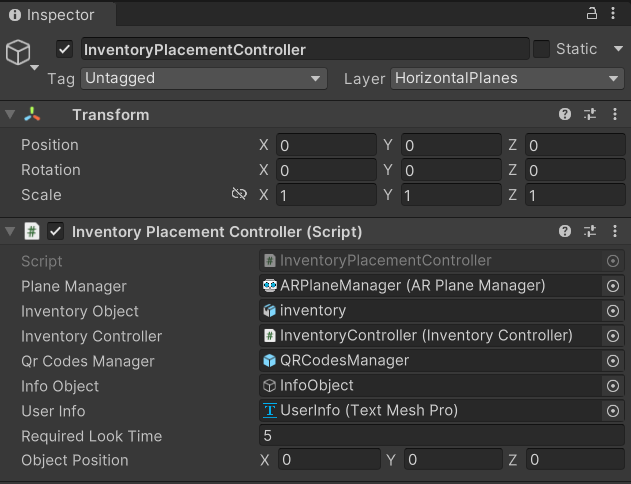
\includegraphics[scale=0.8]{images/invPlace_Editor}
    \caption{Sicht des Benutzers nach Platzierung des Inventars}
    \label{fig:inventoryPlaced}
\end{figure}

\subsection{Inventory Controller Game Objekt}
Das \textit{Inventory Controller} Game Objekt spielt eine entscheidende Rolle bei der Überwachung und Verwaltung des
Inventars in der Augmented Reality (AR)-Anwendung. Durch das angehängte \textit{InventoryController.cs} Script wird die
\textbf{InventoryController} Klasse realisiert. Diese Klasse ist verantwortlich für die Erkennung neuer Gegenstände im
Inventar, die Überprüfung auf verfügbaren Platz im Inventar, die Berechnung der Zellenposition anhand der QR-Code-Koordinaten
und die Speicherung der Positionen dieser Items in einem \textit{2D Array}.

Der Zugriff auf die Begrenzungen (\textit{Bounds}) des Inventarmodells ermöglicht es, ständig zu überwachen, ob der
Benutzer ein neues Element in das Inventar gelegt hat. Dieser Ansatz gewährleistet eine präzise Kontrolle über die
Platzierung von Gegenständen im Inventar.

Das \textit{InventoryController.cs} Script interagiert dabei aktiv mit den AR-Elementen, insbesondere den QR-Codes, um
den Platzbedarf der Gegenstände zu überwachen und ihre Positionen im Inventar festzulegen. Zusätzlich interagiert der
\textit{InventoryController} auch mit dem \textit{KnapsackAlgo} Game Objekt, in dem es das verspeicherte \textit{2D Array}
immer weitergibt um damit rechnen zu können.\\

\begin{figure}[h]
    \centering
    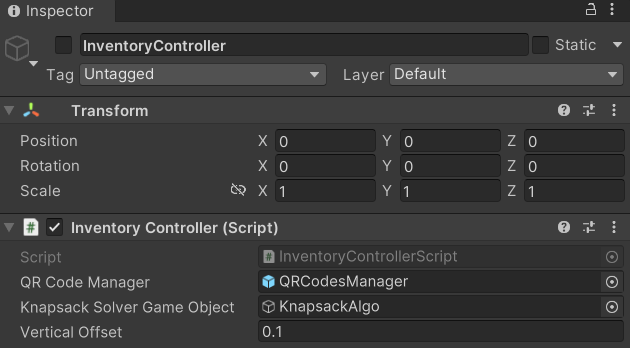
\includegraphics[scale=0.8]{images/invCon_Editor}
    \caption{IventoryController Objekt im Editor}
    \label{fig:InventoryController_Editor}
\end{figure}

Die Abbildung \ref{fig:InventoryController_Editor} zeigt das \textit{iventoryController}-Objekt im Unity Editor.  Hier
können verschiedene Einstellungen vorgenommen werden, darunter die Ebene, in der dieses Objekt liegt, die Koordinaten
im Unity Editor und die angehängte Komponente \textit{InventoryController.cs}. Zudem sind vordefinierte Werte für bestimmte
Variablen sichtbar. Diese Variablen umfassen:

\begin{itemize}
    \item \textbf{QRCodesManager:} Referenz auf das \textit{QRCodesManager} Game Objekt aus der Level 2 Szene.
    \item \textbf{Knapsack Solver Game Objekt:} Referenz auf das \textit{KnapsackAlgo} Game Objekt aus der Level 2 Szene.
    \item \textbf{Vertical Offset:} Float Wert um den die Bounds\footnote{Unity \cite{Bounds}} des Inventory Objekts auf der X-Achso erweitert werden.\\
\end{itemize}

\subsubsection{InventoryController Klassenvariablen}
\begin{lstlisting}[style=csharp, caption={Klassenvariablen der InventoryController Klasse}, label=code:controller_var]
public GameObject QRCodeManager;
public GameObject knapsackSolverGameObject;

private SortedDictionary<System.Guid, GameObject> activeQRObjects;

private GameObject inventoryObject;
public float verticalOffset = 0.1f;
private Bounds inventoryBounds;
private int numRows = 3;
private int numColumns = 3;
private int[,] idGrid;
private KnapsackScript knapsackScript;
private int cap;
private int currWeight = 0;
private string message;
private HashSet<int> processedItems;
\end{lstlisting}
Die gezeigten Klassenvariablen in Codeabschnitt \ref{code:controller_var} sind Teil der \textit{InventoryController} Klasse.
Öffentliche(\textbf{public}) Variablen repräsentieren Objekte und Werte, die im Unity Editor festgelegt und übergeben werden
oder von anderen Klassen für die funktionalität gebraucht werden. Dies ermöglicht einen direkten Zugriff auf diese Objekte in der
eigenen oder einer anderen Klasse. Die float-Variable \textit{verticalOffset} spielt hier eine
wichtige Rolle, für die erweiterung der \textit{Bounds} von dem Inventar Modell. Die privaten (\textbf{private}) Variablen dienen
der lokalen Speicherung von Werten, die von keiner anderen Klasse benötigt werden.\\

\subsubsection{Start des InventoryControllers}
\begin{lstlisting}[style=csharp, caption={Start Funktion des InventoryControllers}, label=code:controller_start]
void Start()
{
    activeQRObjects = QRCodeManager.GetComponent<QRCodesVisualizer>().qrCodesObjectsList;
    knapsackScript = knapsackSolverGameObject.GetComponent<KnapsackScript>();
    cap = knapsackScript.capacity;
    processedItems = new HashSet<int>();
    UpdateInventoryBounds();
    InitializeIDGrid();
}
\end{lstlisting}
Die \textbf{Start()} Funktion wird zu Beginn des Inventory Controllers aufgerufen und aufgeführt. Hier werden die
wichtigen Objekte die für den weiteren Verlauf des Programms notwendig sind deklariert beziehungsweise erstellt und
ebenfalls werden die beiden Funktionen \textbf{UpdateInventoryBounds()} und \textbf{InitializeIDGRid()} aufgerufen.\\

\subsubsection{Neue Bounds setzen}
\begin{lstlisting}[style=csharp, caption={Funktion um Inventar Bounds zu erweitern}, label=code:controller_updateBounds]
private void UpdateInventoryBounds()
{
    if (inventoryObject != null)
    {
        Bounds localBounds = GetBounds(inventoryObject);
        ExtendBounds(ref localBounds, verticalOffset);
        inventoryBounds = localBounds;
    }
}
\end{lstlisting}
Um zu erreichen, dass man ein Item wirklich in die Bounds des Inventars legen kann wird in der \textbf{UpdateInventoryBounds()}
Funktion genau dies ausgeführt. Es werden die aktuellen Bounds des Inventars gespeichert und diese werden dann mittels
der \textbf{ExtendBounds()} Funktion erweitert und anschließend werden diese Bounds als neue Bounds gespeichert.\\

\subsubsection{Bounds des Inventars ermitteln}
\begin{lstlisting}[style=csharp, caption={Funktion um Bounds zu ermitteln}, label=code:controller_getBounds]
private Bounds GetBounds(GameObject obj)
{
    Renderer renderer = obj.GetComponent<Renderer>();
    return renderer != null ? renderer.bounds : new Bounds(obj.transform.position, Vector3.one);
}
\end{lstlisting}
Die von \ref{code:controller_updateBounds} aufgerufene Funktion \textbf{GetBounds()} greift auf den Renderer\footnote{Unity \cite{Renderer}}
des Inventar Modells zu um dadurch auf die Bounds zuzugreifen zu können, denn der Renderer ist dafür verantwortlich,
dass das Modell überhaupt sichtbar ist. Wenn dieser Renderer ungleich \textbf{null} ist, gibt er die neuenn Bounds zurück und speichert
sie in \textit{localBounds} von Codeabschnitt \ref{code:controller_updateBounds}.\\

\subsubsection{Inventory Bounds erweitern}
\begin{lstlisting}[style=csharp, caption={Funktion um Bounds zu erweitern}, label=code:controller_extendBounds]
private void ExtendBounds(ref Bounds bounds, float offset)
{
    bounds.center = new Vector3(bounds.center.x, bounds.center.y + offset / 2, bounds.center.z);
    bounds.extents = new Vector3(bounds.extents.x, bounds.extents.y + offset / 2, bounds.extents.z);
}
\end{lstlisting}
Um anschließend diese Bounds zu erweitern um zu erkennen ob QR-Koordinaten innerhalb von diesen Bounds ist wird die von
\ref{code:controller_updateBounds} aufgerufene Funktion \textbf{ExtendBounds()} ausgeführt. Diese Funktion erzielt, dass die
Bounds von dem Inventar Modell auf der X-Achso um das \textit{Vertical Offset} erweitert werden. Nach Abschluss dieser Funktion
sehen die Bounds von diesem Modell dann folgendermaßen aus:
\begin{figure}[h]
    \centering
    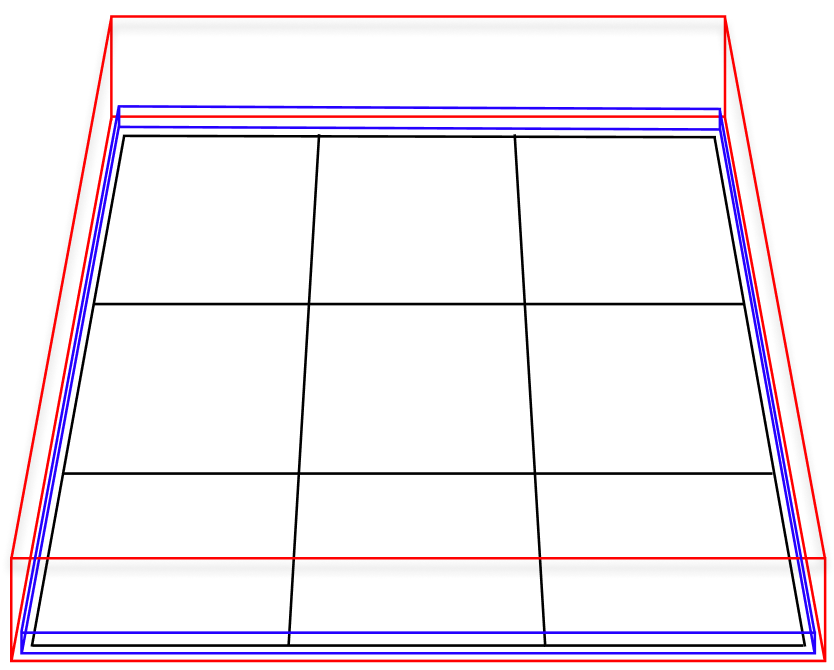
\includegraphics[scale=0.4]{images/extendedBounds}
    \caption{Erweiterte Bounds des Inventar Modells}
    \label{fig:extended_inventoryBounds}
\end{figure}

Auf der Abbildung \ref{fig:extended_inventoryBounds} ist eine einfache schematische Zeichnung des zweidimensionalen Inventars zu sehen. Die
blaue Umrandung repräsentiert die Begrenzungen (Bounds) vor der Ausführung der Funktion \textbf{UpdateInventoryBounds()}
aus dem Codeabschnitt \ref{code:controller_updateBounds}. Nachdem die Funktion ausgeführt wurde, wird die rote Umrandung
dargestellt. Durch die neuen Bounds wird deutlich, dass insbesondere die Begrenzung entlang der X-Achse erweitert wurde.

Die Erweiterung der Bounds ist von entscheidender Bedeutung, da nicht erweiterte Bounds die Höhe der Bauklötze nicht
berücksichtigen würden. Dies könnte dazu führen, dass ein QR-Code, der sich tatsächlich innerhalb der Bounds befindet,
als außerhalb betrachtet wird, wenn die Höhe der Bauklötze nicht angemessen einbezogen wird.

Diese Anpassungen sind wichtig, um sicherzustellen, dass die Begrenzungen des Inventars korrekt erfasst werden und somit
eine präzise Verortung von QR-Codes innerhalb der Augmented-Reality-Anwendung gewährleistet ist.\\

\subsubsection{ID Grid Initialisierung}
\begin{lstlisting}[style=csharp, caption={Initialisierung des idGrids}, label=code:controller_initialize]
private void InitializeIDGrid()
{
    idGrid = new int[numRows, numColumns];
}
\end{lstlisting}
Die in Codeabschnitt \ref{code:controller_start} aufgerufene Funktion initialisiert das idGrid mit \textit{numRows} und
\textit{numColumns} also wird das idGrid als \textit{int [3,3]} initialisiert.\\

\subsubsection{Update Funktion}
\begin{lstlisting}[style=csharp, caption={Initialisierung des idGrids}, label=code:controller_update]
void Update()
{
    UpdateGrid();
}
\end{lstlisting}
Nach Abschluss des Codes aus Codeabschnitt \ref{code:controller_start} wird anschließend die \textit{Lebenszyklusmethode}
\textbf{Update()} ausgeführt. Diese Funktion ruft jeden Frame die \textbf{UpdateGrid()} Funktion auf, auf die im nächsten
Abschnitt genau eingegangen wird.\\

\subsubsection{Funktion für neue Items innerhalb des Bounds}
\begin{lstlisting}[style=csharp, caption={Code fuer ueberpruefen neuer Items im Inventar}, label=code:controller_check]
void UpdateGrid()
{
    lock (activeQRObjects)
    {
        foreach (var item in activeQRObjects.Values)
        {
            QRCode qRCode = item.GetComponent<QRCode>();
            Vector3 worldPosition = item.transform.TransformPoint(qRCode.item.qrData.position);

            if (item != null && inventoryBounds.Contains(worldPosition))
            {
                int itemId = qRCode.item.qrData.id;

                if (!processedItems.Contains(itemId))
                {
                    if (currWeight + qRCode.item.qrData.weight <= cap)
                    {
                        processedItems.Add(itemId);
                        message = " ";
                        Vector2 startGridPosition = CalculateGridPosition(worldPosition);
                        idGrid[(int)startGridPosition.x, (int)startGridPosition.y] = itemId;
                        knapsackScript?.UpdateInfoMesh(message);
                        currWeight += qRCode.item.qrData.weight;
                        EventManager.GridUpdate(idGrid);
                    }
                    else
                    {
                        message = "Item hat zu viel Gewicht!";
                        knapsackScript?.UpdateInfoMesh(message);
                    }
                }
            }
            else if (!inventoryBounds.Contains(worldPosition) && processedItems.Contains(qRCode.item.qrData.id) && ContainsId(qRCode.item.qrData.id))
            {
                int itemId = qRCode.item.qrData.id;
                processedItems.Remove(itemId);
                RemoveItem(itemId);
                currWeight -= qRCode.item.qrData.weight;
                EventManager.GridUpdate(idGrid);
            }
        }
        PrintGrid();
    }
}
\end{lstlisting}
Die vorliegende Funktion, \texttt{UpdateGrid()}, ist maßgeblich für die Überwachung und Verwaltung von neu hinzugefügten
oder entfernten Items im Inventar verantwortlich. Zu Beginn eines jeden Frames wird das \texttt{activeQRObjects}-Dictionary
gesperrt, um Thread-Sicherheit zu gewährleisten. Anschließend erfolgt eine Iteration durch jedes Element in diesem Dictionary
mittels einer \texttt{foreach}-Schleife.\\

Innerhalb dieser Schleife wird für jedes Objekt die zugehörige \texttt{QRCode}-Komponente extrahiert, und die Weltposition
des Objekts wird durch Transformation der lokalen Position des QR-Codes unter Berücksichtigung der Transformation des
übergeordneten Objekts berechnet.\\

Die Hauptüberprüfung erfolgt daraufhin, ob das aktuelle Item nicht null ist und ob seine Weltposition innerhalb der durch
\texttt{inventoryBounds} definierten Grenzen liegt. Wenn diese Bedingungen erfüllt sind, wird das Item als "hinzugefügt"
betrachtet.\\

Im weiteren Verlauf wird überprüft, ob die ID des Items bereits in der Menge der verarbeiteten Items (\texttt{processedItems})
vorhanden ist. Falls nicht, wird überprüft, ob das Hinzufügen des Items das aktuelle Gesamtgewicht (\texttt{currWeight})
zusammen mit dem Gewicht des Items unter die maximale Kapazität (\texttt{cap}) bringt.\\

Wenn diese Bedingungen erfüllt sind, wird das Item in die Menge der verarbeiteten Items aufgenommen, eine Nachricht wird
auf Leer gesetzt, das \textit{currWeight} wird um das Gewicht des verarbeiteten Items erweitertund die Position des
Items im zweidimensionalen Array \texttt{idGrid} wird aktualisiert. Zusätzlich wird die Anzeige des Inventars durch den
Aufruf der Methode \texttt{UpdateInfoMesh} des \texttt{knapsackScript}aktualisiert, und das aktuelle Gewicht des Inventars
wird entsprechend angepasst. Schließlich wird das Event\textbf{GridUpdate()} des \textit{EventManager} ausgelöst. Dieses
Event ist maßgäblich für das Übergeben des \textit{idGrid}and das \textit{knapsackScript} für die weitere Verarbeitung.
\begin{figure}[h]
    \centering
    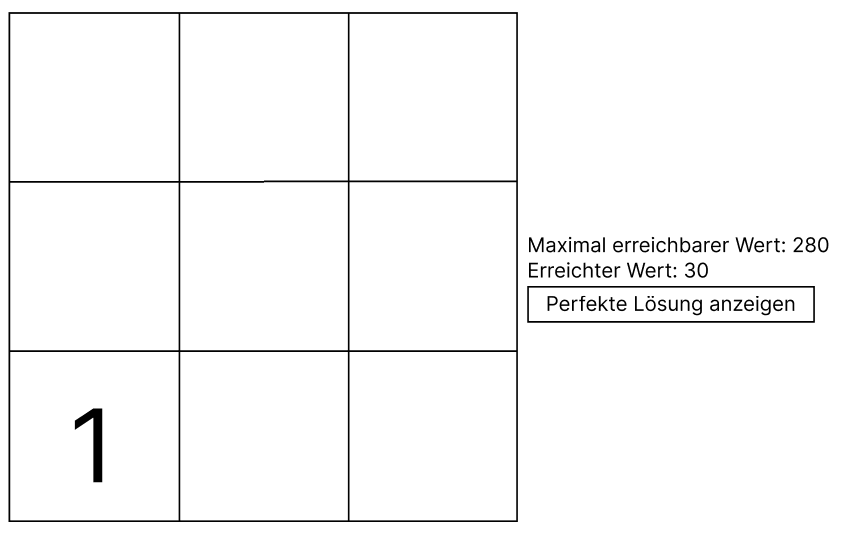
\includegraphics[scale=0.6]{images/itemAdded}
    \caption{Item zu Inventar hinzugefügt}
    \label{fig:controller_itemAdded}
\end{figure}

In Abbildung \ref{fig:controller_itemAdded} ist der Zustand nach dem Hinzufügen eines Items dargestellt. In Zelle 7 wurde
das Item mit der \textit{ID: 1} hinzugefügt. Nach dem Hinzufügen des Items wird der \textit{Knapsack Algorithmus} ausgelöst
und anschließend die beiden TextMehes aktualisiert, indem in dem oberen TextMesh der maximal erreichbare Wert angezeigt wird
und in dem unteren der Wert des selbst zusammengestellten Inventars.\\

Nachdem das Item im Inventar platziert wurde sieht nun dass \textit{idGrid} folgendermaßen aus:
\begin{lstlisting}[style=csharp, caption={ID verspeichert}, label=code:controller_savedID]
int idGrid = [[0, 0, 0],
              [0, 0, 0],
              [1, 0, 0]];
\end{lstlisting}\\

Das Hashset \textit{processedItems} sieht nach platzieren des Items dann so aus:
\begin{lstlisting}[style=csharp, caption={ID verspeichert}, label=code:controller_savedID]
processedItems = [1];
\end{lstlisting}\\

Sollte das Gewicht des hinzugefügten Items die Kapazität überschreiten, wird eine Fehlermeldung generiert, und die
Aktualisierung des Grids wird unterbunden. Die Fehlermeldung und der resultierende Zustand des Grids sind in Abbildung
\ref{fig:controller_itemToHeavy} dargestellt.
\begin{figure}[h]
    \centering
    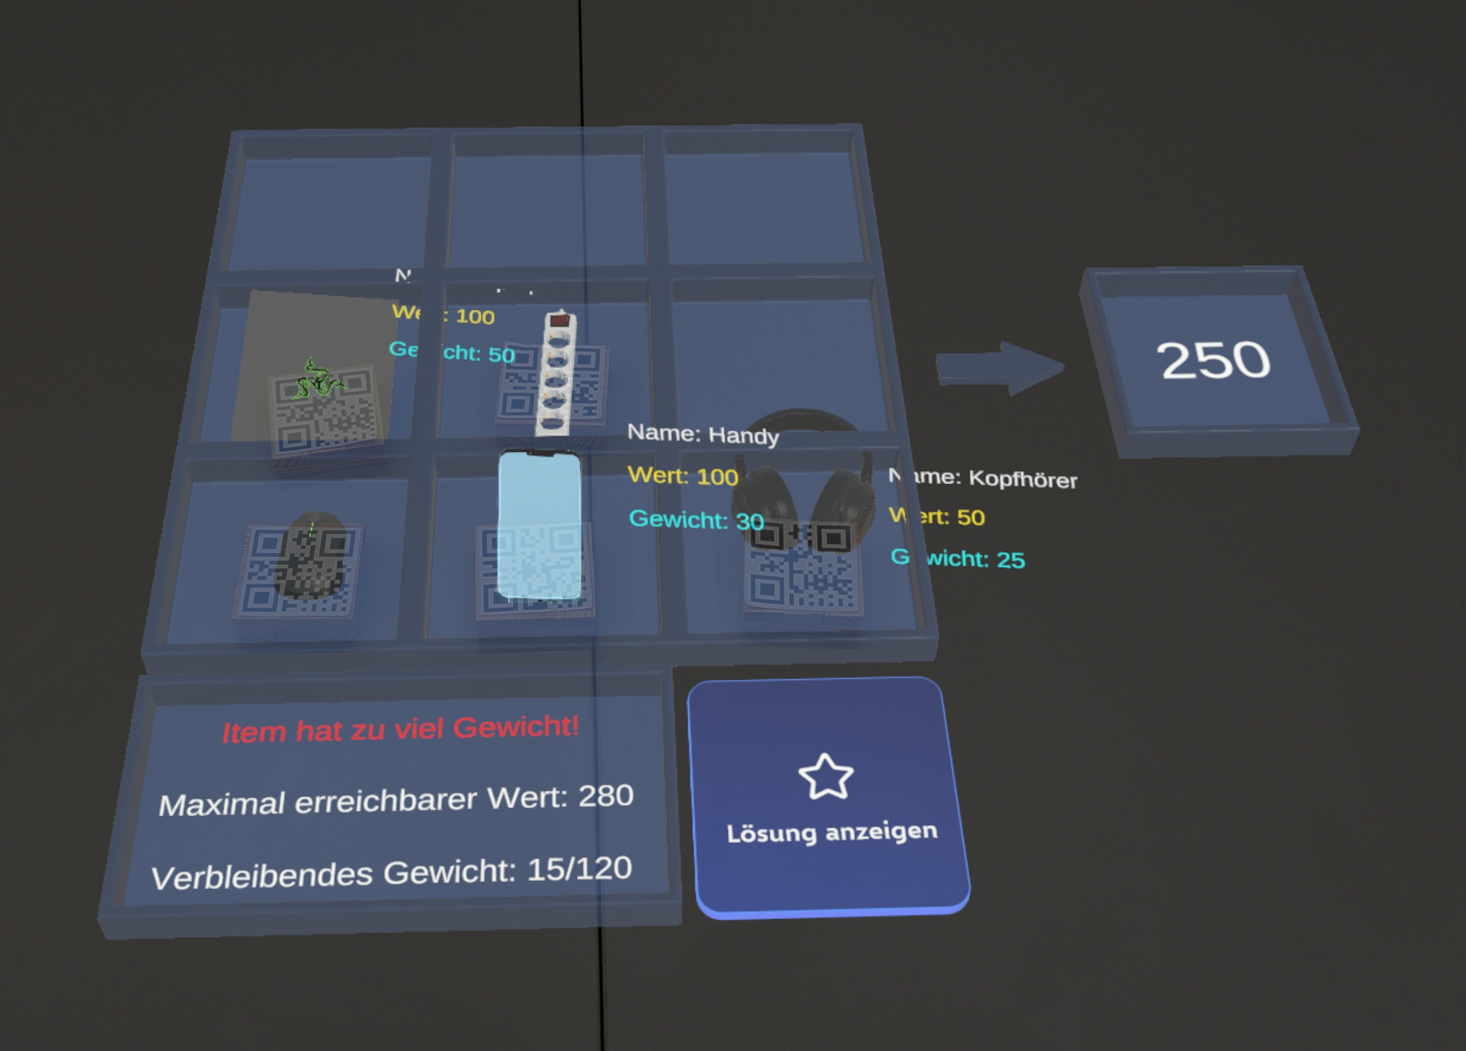
\includegraphics[scale=0.6]{images/itemToHeavy}
    \caption{Item zu schwer}
    \label{fig:controller_itemToHeavy}
\end{figure}

In Abbildung \ref{fig:controller_itemToHeavy} sind vier verschiedene Items im Inventar enthalten, mit den IDs
\textit{1, 3, 5, 9}. Die Reihenfolge ihres Hinzufügens zum Inventar war 1, 5, 9, 3. Das Item mit der ID 9 wurde jedoch
aufgrund seines zu hohen Gewichts nicht zu \textit{idGrid} und \textit{processedItems} hinzugefügt. Gleichzeitig wird
eine Fehlermeldung angezeigt, um dem Benutzer zu signalisieren, dass das zuletzt hinzugefügte Item zu schwer für das
aktuelle Inventar ist. Als Konsequenz bleiben \textit{idGrid} und \textit{processedItems} unverändert und enthalten
daher nicht die ID 9. Im Hintergrund sieht daher das \textit{idGrid} dementsprechend folgendermaßen aus:
\begin{lstlisting}[style=csharp, caption={Item zu schwer fuer das Inventar}, label=code:controller_savedIDs]
int idGrid = [[0, 0, 0],
              [5, 0, 0],
              [1, 3, 0]];
\end{lstlisting}\\
Das HashSet \textit{processedItems} sieht nach platzieren des Items dann so aus:
\begin{lstlisting}[style=csharp, caption={ID verspeichert}, label=code:controller_savedID]
processedItems = [1, 5, 9];
\end{lstlisting}\\
Sobald der Benutzer dieses Item wieder aus dem Inventar entfernt wird die Fehlermeldung nicht mehr angezeigt und es kann
ein passendes Item hinzugefügt werden.\\

Im alternativen Zweig der Hauptbedingung wird überprüft, ob das Item außerhalb der Inventargrenzen liegt, aber zuvor
als verarbeitet markiert wurde und weiterhin in \texttt{processedItems} und \texttt{idGrid} vorhanden ist. Dies deutet
darauf hin, dass das Item aus dem Inventar entfernt wurde. In diesem Fall wird die ID des Items aus \texttt{processedItems}
und \texttt{idGrid} entfernt, und das Gewicht des Inventars wird entsprechend angepasst. Auch hier wird ein
\texttt{GridUpdate}-Ereignis ausgelöst.\\

\begin{figure}[h]
    \centering
    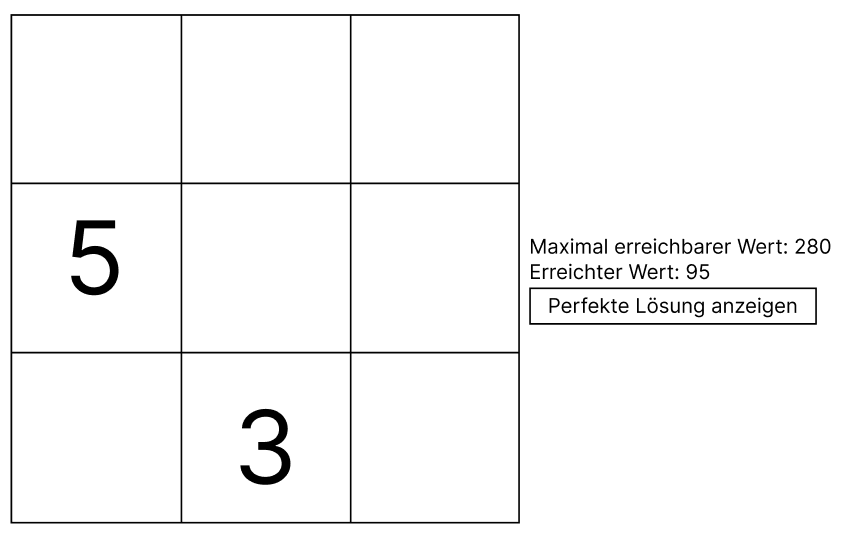
\includegraphics[scale=0.6]{images/itemEntfernt}
    \caption{Item aus Inventar entfernt}
    \label{fig:controller_itemEntfernt}
\end{figure}

In Abbilding \ref{fig:controller_itemEntfernt} ist der aktuelle Zustand eines selbst zusamengestellten Inventars zu sehen. In
diesem Inventar sind die beiden Items mit den IDs \textit{5, 3} enthalten. Im Hintergrund sieht das \textit{idGrid} jedoch so aus:
\begin{lstlisting}[style=csharp, caption={ID trotz nicht vorhandenem Item gespeichert}, label=code:controller_savedIDitemEntferntGrid]
int idGrid = [[0, 0, 0],
              [5, 0, 0],
              [1, 3, 0]];
\end{lstlisting}\\
Und das HashSet \textit{processedItems} sieht so aus:
\begin{lstlisting}[style=csharp, caption={ID trotz nicht vorhandenem Item gespeichert}, label=code:controller_savedIDItemEntferntHash]
processedItems = [1, 5, 3];
\end{lstlisting}\\
Anhand der Abbildung \ref{fig:controller_itemEntfernt} und den beiden Codeabschnitten \ref{code:controller_savedIDitemEntferntGrid}
und \ref{code:controller_savedIDItemEntferntHash} ist aber zu sehen, dass hier noch die ID \textit{1} gespeichert ist.
Dies bedeutet, dass das Item mit der ID \textit{1} in einem vorherigen Zustand im Inventar platziert wurde aber jetzt außerhalb
der Bounds des Iventars liegt. Anhand dieser Erkenntnis wird anschließend diese ID aus dem \textit{idGrid} und \textit{processedItems}
entfernt und das \textit{currWeight} angepasst. Diese sehen nach der Entfernung dieser ID folgendermaßen aus:
\begin{lstlisting}[style=csharp, caption={ID trotz nicht vorhandenem Item gespeichert}, label=code:controller_savedIDgg]
int idGrid = [[0, 0, 0],
              [5, 0, 0],
              [0, 3, 0]];
\end{lstlisting}
\begin{lstlisting}[style=csharp, caption={ID verspeichert}, label=code:controller_savedIDID]
processedItems = [5, 3];
\end{lstlisting}\\
Schließlich erfolgt der Aufruf der Funktion \textbf{PrintGrid()}, die Testweise für das Debugging enthalten ist
um aus den Logs herauslesen zu können, wie das \textit{idGrid} aufgebaut ist und welche Items enthalten sind und ob
die Berechnung und Platzierung richtig abgelaufen ist.

\subsubsection{Berechnen der Position im idGrid anhand der Koordinaten}
In Codeabschnitt \ref{code:controller_check} wird bei platzieren eines Items innerhalb des Inventars die Funktion
\textbf{CalculateGridPosition()} aufgerufen. Diese Funktion kümmert sich darum, dass anhand der gegebenen Koordinaten des
Items innerhalb des Inventar Modells ein Vektor Berechnet wird an welcher Stelle dieses Item im \textit{idGrid} liegt.
Diese Funktion sieht folgendermaßen aus:
\begin{lstlisting}[style=csharp, caption={Stelle im idGrid anhand Koordinaten berechnen}, label=code:controller_calcPos]
private Vector2 CalculateGridPosition(Vector3 objectPosition)
{
    float cellWidth = inventoryBounds.size.x / numColumns;
    float cellHeight = inventoryBounds.size.z / numRows;
    int col = Mathf.FloorToInt((objectPosition.x - inventoryBounds.min.x) / cellWidth);
    int row = Mathf.FloorToInt((inventoryBounds.max.z - objectPosition.z) / cellHeight);
    return new Vector2(row, col);
}
\end{lstlisting}\\
Die Funktion beginnt damit, dass sie sich anhand der Länge der Bounds in X- und Y-Achse die Länge einer einzelnen Zelle
berechnet. Die Variable \texttt{cellWidth} repräsentiert die Breite jeder Zelle, und \texttt{cellHeight} repräsentiert
die Höhe jeder Zelle im Inventar-Raster.

Anschließend werden die 2D-Koordinaten der Position des übergebenen Objekts im Inventar-Raster berechnet. Dazu wird
zuerst die X-Koordinate des Objekts relativ zur minimalen X-Grenze der Inventar-Bounds genommen und durch die Breite
einer Zelle (\texttt{cellWidth}) geteilt. Dieser Wert wird dann auf die nächste ganze Zahl abgerundet
(\texttt{Mathf.FloorToInt}) und repräsentiert die Spalte (\texttt{col}) im Raster.

Ebenso wird die Z-Koordinate des Objekts relativ zur maximalen Z-Grenze der Inventar-Bounds genommen und durch die Höhe
einer Zelle (\texttt{cellHeight}) geteilt. Auch dieser Wert wird auf die nächste ganze Zahl abgerundet und repräsentiert
die Zeile (\texttt{row}) im Raster.

Abschließend werden die berechneten Zeilen- und Spaltenwerte als 2D-Vektor (\texttt{Vector2}) zurückgegeben, der die
Position des Objekts im Inventar-Raster repräsentiert.

\subsubsection{Hilfsfunktionen}
Im Codeabschnitt \ref{code:controller_check} werden die Funktionen \textbf{RemoveItem} und \textbf{ContainsID} für die
Entfernung eines Items aus dem \textit{idGrid} und die Überprüfung, ob eine bestimmte Item-ID im \textit{idGrid}
vorhanden ist, verwendet. Die Funktion \textbf{RemoveItem} hat den Zweck, ein Item anhand seiner ID aus dem \textit{idGrid} zu entfernen.
Die Funktion \textbf{ContainsID} wird verwendet, um zu überprüfen, ob eine bestimmte Item-ID bereits im \textit{idGrid}
vorhanden ist. Die Implementierungen dieser Funktionen sind entsprechend:
\begin{lstlisting}[style=csharp, caption={ID aus idGrid entfernen}, label=code:controller_removeID]
private void RemoveItem(int id)
{
    for (int i = 0; i < numRows; i++)
    {
        for (int j = 0; j < numColumns; j++)
        {
            if (idGrid[i, j] == id)
            {
                idGrid[i, j] = 0;
                return;
            }
        }
    }
}
\end{lstlisting}\\
\begin{lstlisting}[style=csharp, caption={Ueberpruefen ob ID in idGrid enthalten ist}, label=code:controller_contains ID]
private bool ContainsId(int id)
{
    for (int i = 0; i < numRows; i++)
    {
        for (int j = 0; j < numColumns; j++)
        {
            if (idGrid[i, j] == id)
            {
                return true;
            }
        }
    }
    return false;
}
\end{lstlisting}\\

%HIER EVENTMANAGER EINBAUEN HIHI

\subsection{Knapsack Solver Game Objekt}
Das \textit{Knapsack Solver} Game Objekt spielt die Hauptrolle um Berechnungn durchzuführen.
Durch das angehängte \textit{KnapsackSolver.cs} Script wird die \textit{KnapsackSolver} Klasse reasliert. Diese
Klasse ist verantworlich für die Berechnung der perfekten Lösung und ebenfalls für die Berechnung des selbst
zusammengestellten Inventars des Benutzers.

Durch die Interaktion zwischen der \textit{InventoryController}, der \textit{KnapsackScript} Klasse und der
\textit{EventManager} Klasse wird bei jedem neuen Item stets gewährleistet, dass das Inventar mit dem gerechnet wird
stets das aktuelle ist.\\

\begin{figure}[h]
    \centering
    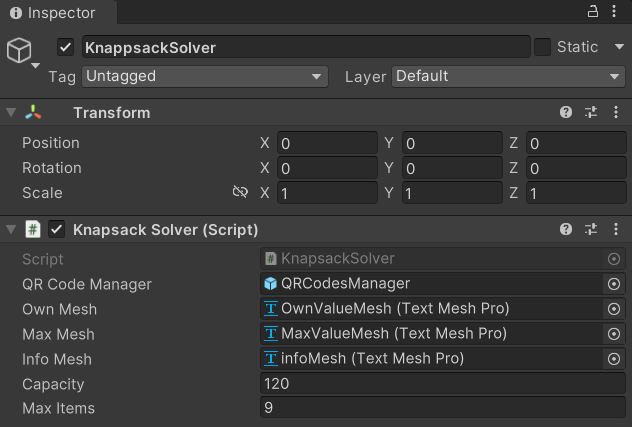
\includegraphics[scale=0.8]{images/knapsackEditor}
    \caption{Knapsack Algorithmus Objekt im Editor}
    \label{fig:Knapsack_Editor}
\end{figure}

Die Abbildung \ref{fig:Knapsack_Editor} zeigt das \textit{KnapsackAlgo}-Ojekt im Unity Editor. Hier können verschiedene
Einestellungen vorgenommen werden, darunter die Ebene, in der dieses Objekt liegt, die Koordinaten des Objekts im
Unity Editor selbst und die angehängte Komponente \textit{KnapsackScript.cs}. Zudem sind vordefinierte Werte für
bestimmte Variablen sichtbar. Diese Variablen umfassen:

\begin{itemize}
    \item \textbf{QRCodesManager:} Referenz auf das \textit{QRCodesManager} Game Objekt aus der Level 2 Szene.
    \item \textbf{Own Mesh:} Referenz auf das \textit{OwnValueMesh} aus dem \textit{infoObjekt} aus der Level 2 Szene.
    \item \textbf{Max Mesh:} Referenz auf das \textit{MaxValueMesh} aus dem \textit{infoObjekt} aus der Level 2 Szene.
    \item \textbf{Info Mesh:} Referenz auf das \textit{infoMesh} aus dem \textit{infoObjekt} aus der Level 2 Szene.
    \item \textbf{Capacity:} Integer Wert der die Kapazität für den \textit{Knapsack Algorithmus} festlegt.
    \item \textbf{Max Items:} Repräsentiert die maximale Anzahl an Items die in das Inventar gelegt werden können. Dies
    dient als extra Bedingung für den \textit{Knapsack Algorithmus}.\\
\end{itemize}

\subsubsection{Klassenvariablen KnapsackScript}
\begin{lstlisting}[style=csharp, caption={Klassenvariablen des KnapsackSolvers}, label=code:Klassenvariablen_kn]
public GameObject QRCodeManager;
public TextMeshPro ownMesh;
public TextMeshPro maxMesh;
public TextMeshPro infoMesh;

public int[,] usedItems;
public int capacity = 120;
public Dictionary<int, QRData> items;
public int maxItems = 9;

private int[,] inventory;
\end{lstlisting}\\
Die in Codeabschnitt \ref{code:Klassenvariablen_kn} präsentierten Klassenvariablen gehören zur Klasse \textit{KnapsackScript}.
Öffentliche (\textbf{public}) Variablen repräsentieren Objekte und Werte, die im Unity Editor festgelegt und übergeben
werden oder von anderen Klassen für die Funktionalität benötigt werden. Diese Bereitstellung ermöglicht einen direkten
Zugriff auf diese Objekte in der eigenen oder einer anderen Klasse. Das \textit{2D int Array inventory} spielt eine
entscheidende Rolle bei der Verarbeitung und Berechnung des Werts des individuellen Inventars.\\

\subsubsection{Start des KnapsackScripts}
\begin{lstlisting}[style=csharp, caption={Start Funktion des KnapsackScripts}, label=code:kn_start]
void Start()
{
    items = new QRItem(0).items;
    EventManager.OnGridUpdate += SetInventory;
}
\end{lstlisting}\\
In dem Codeabschnitt \ref{code:kn_start} ist die Lebenszyklusfunktion \textbf{Start()} zu sehen. Diese Funktion versichert
das erfolgreiche setzen aller Items in dem \textit{Items-Dictionary} und ebenfalls, dass wenn im \textit{EventManager}
das \textit{OnGridUpdate} Event ausgelöst wurde, dass die \textbf{SetInventory()} Funktion aufgerufen wird.

\subsubsection{Set Inventory und Start der Berechnung}
\begin{lstlisting}[style=csharp, caption={Setzen des Inventars und starten der Berechnung}, label=code:kn_setInv]
public void SetInventory(int[,] newInventory)
{
    inventory = newInventory;
    CalculateKnapsack();
}
\end{lstlisting}\\
Die in Codeabschnitt \ref{code:kn_setInv} vom \textit{EventManager} aufgerufene Funktion \textbf{SetInventory}
kümmert sich darum, dass das von dem \textit{InventoryController} zusammengestellte Inventar an das \textit{KnapsackScript}
übergeben wird und ruft anschließend die \textbf{CalculateKnapsack()} Funktion auf, die die Berechnung startet.

\subsubsection{Start der Berechnung}
\begin{lstlisting}[style=csharp, caption={Start der Berechnung}, label=code:kn_startCalc]
void CalculateKnapsack()
{
    int maxValue = KnapsackMaxValue(out usedItems);
    int inventoryValue = -1;
    maxMesh.text = "Maximal erreichbarer Wert: " + maxValue.ToString();
    try
    {
        inventoryValue = KnapsackInventoryValue(inventory);
        if (maxValue == inventoryValue)
        {
            infoMesh.color = Color.green;
            infoMesh.text = "Maximale Punktzahl erreicht";
        }
        else
        {
            infoMesh.text = "";
        }
        ownMesh.text = "Erreichter Wert: " + inventoryValue.ToString();

    }
    catch (Exception e)
    {
        Debug.LogError("Error calculating inventory value: " + e.Message);
    }
}
\end{lstlisting}\\
Um jetzt den Knapsack Algorithmus zu starten und ebenfalls den Wert des eigenen Inventars zu berechnen wird in Codeabschnitt
\ref{code:kn_startCalc} zu begin der Integer Wert \textit{maxValue} definiert. Dieser Wert wird dann mittels der Funktion
\textbf{KnapsackMaxValue} befüllt. Anschließend wird der Text von dem \textit{maxMesh} gesetzt um diesen Wert dem Benutzer
anzuzeigen.

Um jegliche Fehler bei der Berechnung des eigenen Inventars zu vermeiden wird vor der tatsächlichen Berechnung des eigenen
Inventars das \textit{inventoryValue} auf -1 gesetzt um im Fehlerfall einen Program-Cash zu vermeiden.
Anschließend wird jetzt in einem \textit{Try/Catch} Block der Wert des eigenen Inventars mittels der \textbf{KnapsackInvenotryValue}
Funktion berechnet. Anschließend werden mehrere Überprüfungen durchlaufen um zu überprüfen ob der Benutzer den maximal erreichbaren
Wert erzielt hat oder nicht. Wenn dies der Fall ist wird in dem \textit{infoMesh} angezeigt, dass der maximale Wert erreicht wurde.
Wenn dies aber nicht der Fall ist wird einfach der erreichte Wert angezeigt ohne zusätzliche Informationen\\

\subsubsection{Wert des eigenen Inventars}
\begin{lstlisting}[style=csharp, caption={Wert des selbst zusammengestellten Inventars berechnen}, label=code:kn_startCalcOwn]
public int KnapsackInventoryValue(int[,] inventory)
{
    if (inventory == null)
    {
        throw new System.Exception("Inventory is null");
    }

    int totalValue = 0;

    foreach (var item in items.Values)
    {
        int itemId = item.id;
        int itemValue = item.value;

        for (int j = 0; j < inventory.GetLength(0); j++)
        {
            for (int k = 0; k < inventory.GetLength(1); k++)
            {
                if (inventory[j, k] == itemId)
                {
                    totalValue += itemValue;
                }
            }
        }
    }

    return totalValue;
}
\end{lstlisting}\\
Die in Codebaschnitt \ref{code:kn_startCalc} aufgerufene Funktion \textbf{KnapsackInventoryValue()} ist hier in Codebaschnitt
\ref{code:kn_startCalcOwn} zu sehen. Zu Start dieser Funktion wird überprüft ob das Inventar \textit{null} ist um zusätzliche
Sicherheit zu gewhärleisten, falls irgendwo ein Fehler unterläuft. In diesem Fall wird dann eine \textit{System Exception}
geworfen.

Wenn kein Fehler geworfen wird, wird anschließend ein Integer Wert \textit{totalValue} mit 0 initialisiert. Nun werden allen
Items die in dem \textit{items} dictionary vorhanden sind mit einer \textit{foreach} Schleife durchlaufen und bei jedem
Durchlauf wird von diesem Item die \textit{id} und das \textit{value} gespeichert. Der letzte Schritt ist jetzt mit
einer \textit{for}-Schleife durch das \textit{inventory} zu iterieren und and der Stelle \textit{inventory[i,k]} zu überprüfen
ob die id an dieser Stelle des Inventars gleich der id des aktuellen Items ist. Wenn das der Fall ist wird das Value des
Items zu dem \textit{totalValue} dazu addiert.

Nach Abschluss der \textit{foreach}-Schleife wird nun das kalkulierte \textit{totalValue} zurückgegeben.\\

\subsubsection{Knapsack Algorithmus Definition}
Im folgenden Abschnitt wird der Knapsack-Algorithmus allgemein erklärt, die Problemstellung verdeutlicht und die
Unterschiede der beiden möglichen Algorithmen erläutert. Außerdem wird darauf eingegangen, warum er so wichtig ist
und in welchen Anwendungen er zum Einsatz kommt.

Der Knapsack-Algorithmus ist ein häufig verwendetes Werkzeug in der Informatik, um das Problem der optimalen
Ressourcenallokation zu lösen. Dieses Problem tritt auf, wenn eine begrenzte Menge an Ressourcen so effizient wie
möglich genutzt werden soll, um einen bestimmten Nutzen oder Gewinn zu maximieren. Der Begriff "Knapsack" leitet sich
von der Idee ab, dass man versucht, einen Rucksack mit begrenztem Fassungsvermögen mit Gegenständen zu füllen, die
unterschiedliche Werte und Gewichte haben.

\subsubsection{Problemstellung}
Gegeben sei ein Rucksack mit begrenzter Kapazität und eine Menge von Gegenständen, von denen jeder einen bestimmten
Wert und ein bestimmtes Gewicht hat. Das Ziel besteht darin, die Gegenstände auszuwählen, die in den Rucksack passen
und den Gesamtwert maximieren.

\subsubsection{Algorithmus}
Der Knapsack-Algorithmus kann in verschiedenen Varianten implementiert werden, darunter der dynamische
Programmieransatz und der Greedy-Ansatz. Im dynamischen Programmieransatz wird eine Tabelle erstellt, um
Teilprobleme zu lösen und die optimale Lösung zu berechnen. Der Greedy-Ansatz hingegen wählt Gegenstände basierend
auf bestimmten Kriterien aus, um eine lokale Optimierung zu erreichen.

In unserem Kontext wurde der dynamische Programmieransatz implementiert, um den Knapsack-Algorithmus umzusetzen.
Der Code dafür ist in der Datei \textit{KnapsackScript.cs} zu finden, welche den maximal erreichbaren Wert und
die optimale Lösung berechnet.

\subsubsection{Anwendungen}
Der Knapsack-Algorithmus findet Anwendung in verschiedenen Bereichen, darunter Logistik, Finanzplanung,
Ressourcenmanagement und Netzwerkoptimierung. Beispielsweise kann er verwendet werden, um den effizientesten
Transport von Gütern mit begrenzten Kapazitäten zu planen oder in der Finanzplanung, um das Portfolio von
Investitionen zu optimieren.

\subsubsection{Knapsack Algorithmus Implementierung}
Der folgende Abschnitt beschreibt die \textbf{KnapsackMaxValue()} Funktion die den maximal erreichbaren Wert berechnet
und zusätzlich einer der vielen perfekten Lösungen speichert um sie später anzeigen zu können.\\

\begin{lstlisting}[style=csharp, caption={Knapsack Algorithmus / Item Backtracking}, label=code:startKnapsack]
public int KnapsackMaxValue(out int[,] usedItems)
{
    int n = items.Count;
    int[,] dp = new int[n + 1, capacity + 1];
    bool[,] selected = new bool[n + 1, capacity + 1];

    for (int i = 0; i <= n; i++)
        {
        for (int w = 0; w <= capacity; w++)
            {
            if (i == 0 || w == 0)
            dp[i, w] = 0;
            else if (i <= maxItems && items[i].weight <= w)
                {
                int newValue = items[i].value + dp[i - 1, w - items[i].weight];
                if (newValue > dp[i - 1, w])
                    {
                    dp[i, w] = newValue;
                    selected[i, w] = true;
                }
                else
                    {
                    dp[i, w] = dp[i - 1, w];
                    selected[i, w] = false;
                }
            }
            else
                {
                dp[i, w] = dp[i - 1, w];
                selected[i, w] = false;
            }
        }
    }

    // Backtrack to find selected items
    int[,] tempUsedItems = new int[3, 3];
    int row = n;
    int col = capacity;
    int rowIndex = 0;
    int colIndex = 0;

    while (row > 0 && col > 0 && rowIndex < 3 && colIndex < 3)
        {
        if (selected[row, col] && colIndex < maxItems)
            {
            tempUsedItems[rowIndex, colIndex] = items[row].id;
            col -= items[row].weight;
            row--;

            colIndex++;
            if (colIndex >= 3)
                {
                colIndex = 0;
                rowIndex++;
            }
        }
        else
            {
            row--;
        }
    }

    usedItems = tempUsedItems;

    return dp[n, capacity];
}
\end{lstlisting}\\
\begin{enumerate}
    \item \textbf{Initialisierung der Matrizen:}
    \begin{itemize}
        \item Die Funktion beginnt mit der Initialisierung der Matrizen \textit{dp}, \textit{selected} und \textit{n}
        \item \textit{dp[i, w]} repräsentiert den maximalen Gesamtwert mit den ersten \textit{i} Gegenständen und einer begrenzten Kapazität von \textit{w}.
        \item \textit{selected[i, w]} gibt an, ob der Gegenstand \textit{i} in der optimalen Auswahl enthalten ist.
        \item \textit{n} ist die Anzahl der Items, die im \textit{items}-Dictionary enthalten sind.
    \end{itemize}

    \[
        \text{Initialisierung der }\textbf{dp}\text{-Matrix:}
        \begin{bmatrix}
            0 & 0 & \cdots & 0 \\
            0 & 0 & \cdots & 0 \\
            \vdots & \vdots & \ddots & \vdots \\
            0 & 0 & \cdots & 0 \\
        \end{bmatrix}
    \]

    \[
        \text{Initialisierung der }\textbf{selected}\text{-Matrix:}
        \begin{bmatrix}
            \text{false} & \text{false} & \cdots & \text{false} \\
            \text{false} & \text{false} & \cdots & \text{false} \\
            \vdots & \vdots & \ddots & \vdots \\
            \text{false} & \text{false} & \cdots & \text{false} \\
        \end{bmatrix}
    \]

    \item \textbf{Füllen der Matrizen:}
    \begin{itemize}
        \item Die äußere Schleife iteriert über die Gegenstände (\textit{i}), und die innere Schleife über die Kapazitäten des Rucksacks (\textti{w}).
        \item Der Wert in der \textit{dp}-Matrix wird durch den Vergleich zweier Möglichkeiten aktualisiert:
        \begin{enumerate}
            \item Wert des aktuellen Gegenstands + Wert mit verbleibender Kapazität nach Abzug des aktuellen Gegenstands.
            \item Wert ohne Einbeziehung des aktuellen Gegenstands.\\
        \end{enumerate}
        Hier wird entschieden, ob es vorteilhafter ist, den aktuellen Gegenstand einzuschließen oder nicht.
    \end{itemize}

    \[
        \text{Aktualisierte }\textbf{dp}\text{-Matrix:}
        \begin{bmatrix}
            a11 & a12 & \cdots & a15 & a16 & \cdots & a19 & \cdots & a1n \\
            a21 & a22 & \cdots & a25 & a26 & \cdots & a29 & \cdots & a2n \\
            a31 & a32 & \cdots & a35 & a36 & \cdots & a39 & \cdots & a3n \\
            \vdots & \vdots & \ddots & \vdots & \vdots & \ddots & \vdots & \ddots & \vdots \\
            am1 & am2 & \cdots & am3 & am6 & \cdots & am9 & \cdots & \text{MaxValue} \\
        \end{bmatrix}
    \]

    \[
        \text{Aktualisierte }\textbf{selected}\text{-Matrix:}
        \begin{bmatrix}
            \text{false} & \text{false} & \cdots & \text{false} & \text{false} & \cdots & \text{true} \\
            \text{false} & \text{false} & \cdots & \text{true} & \text{false} & \cdots & \text{true} \\
            \vdots & \vdots & \ddots & \vdots & \vdots & \ddots & \vdots \\
            \text{false} & \text{false} & \cdots & \text{true} & \text{false} & \cdots & \text{true} \\
        \end{bmatrix}
    \]

    \item \textbf{Backtracking:}
    \begin{itemize}
        \item Nach dem Füllen der Matrizen erfolgt der Backtracking-Schritt, um die ausgewählten Gegenstände zu ermitteln.
        \item Beginnend von \textit{dp[n, capacity]} (maximaler Wert) wird rückwärts durch die \textit{selected}-Matrix
        navigiert, um die ausgewählten Gegenstände zu identifizieren.
    \end{itemize}

    \item \textbf{Speicherung der ausgewählten Gegenstände:}
    \begin{itemize}
        \item Die ausgewählten Gegenstände werden in der Matrix \textit{tempUsedItems} gespeichert.
        \item \textit{usedItems} bekommt die Werte von \textit{tempUsedItems}.
    \end{itemize}

    \item \textbf{Rückgabe des Ergebnisses:}
    \begin{itemize}
        \item Die Funktion gibt den maximal erreichbaren Gesamtwert zurück.\\
    \end{itemize}
\end{enumerate}

\subsubsection*{Knapsack Beispiel}
Betrachten wir das Knapsack-Problem, bei dem ein Rucksack mit begrenzter Kapazität optimal gefüllt werden soll, um den
Gesamtwert der enthaltenen Gegenstände zu maximieren. Die Kapazität des Rucksacks beträgt \textit{13}. Die Liste der
verfügbaren Gegenstände ist wie folgt definiert:
\begin{center}
\begin{array}{|c|c|c|c|}
    \hline
    \text{ID} & \text{Name} & \text{Gewicht} & \text{Wert} \\
    \hline
    1 & \text{Laptop} & 5 & 10 \\
    2 & \text{Router} & 2 & 5 \\
    3 & \text{Maus} & 2 & 3 \\
    4 & \text{Block} & 1 & 2 \\
    5 & \text{Stifte} & 1 & 1 \\
    6 & \text{Kopfhörer} & 3 & 5 \\
    7 & \text{Taschenrechner} & 1 & 1 \\
    8 & \text{Redbull} & 1 & 5 \\
    9 & \text{USB-Stick} & 1 & 2 \\
    10 & \text{Verteiler} & 2 & 2 \\
    11 & \text{Handy} & 3 & 10 \\
    \hline
\end{array}
\end{center}
\\
Nach Anwendung der dynamischen Programmierung, um die maximale Werttabelle und die Tabelle der ausgewählten Items zu
erstellen sieht die \textit{dp}-Matrix dementsprechend so aus:
\[
    \text{dp-Matrix:}
    \begin{bmatrix}
        0 & 0 & 0 & 0 & 0 & 0 & \cdots & 0 & 0 & 0 \\
        0 & 0 & 0 & 0 & 0 & 10 & \cdots & 10 & 10 & 10 \\
        0 & 0 & 5 & 5 & 5 & 10 & \cdots & 15 & 15 & 15 \\
        0 & 0 & 5 & 5 & 8 & 10 & \cdots & 18 & 18 & 18 \\
        0 & 2 & 5 & 7 & 8 & 10 & \cdots & 20 & 20 & 20 \\
        0 & 2 & 5 & 7 & 8 & 10 & \cdots & 21 & 21 & 21 \\
        0 & 2 & 5 & 7 & 8 & 10 & \cdots & 22 & 23 & 25 \\
        0 & 2 & 5 & 7 & 8 & 10 & \cdots & 22 & 23 & 25 \\
        0 & 5 & 7 & 10 & 12 & 13 & \cdots & 23 & 27 & 28 \\
        0 & 5 & 7 & 10 & 12 & 14 & \cdots & 25 & 27 & 29 \\
        0 & 5 & 7 & 10 & 12 & 14 & \cdots & 25 & 27 & 29 \\
        0 & 5 & 7 & 10 & 12 & 14 & \cdots & 25 & 27 & 29 \\
    \end{bmatrix}
\]
\\
Die zugehörige \textit{selected}-Matrix für die \textit{ausgewählten Gegenstände} lautet:
\[
    \text{selected-Matrix:}
    \begin{bmatrix}
        0 & 0 & 0 & 0 & 0 & 0 & \cdots & 0 & 0 & 0 \\
        0 & 0 & 0 & 0 & 1 & 1 & \cdots & 1 & 1 & 1 \\
        0 & 0 & 1 & 1 & 0 & 0 & \cdots & 1 & 1 & 1 \\
        0 & 0 & 0 & 0 & 0 & 0 & \cdots & 1 & 1 & 1 \\
        0 & 1 & 0 & 1 & 0 & 1 & \cdots & 1 & 1 & 1 \\
        0 & 0 & 0 & 0 & 0 & 0 & \cdots & 0 & 1 & 1 \\
        0 & 0 & 0 & 0 & 0 & 0 & \cdots & 0 & 1 & 1 \\
        0 & 0 & 0 & 0 & 0 & 0 & \cdots & 0 & 0 & 0 \\
        0 & 1 & 1 & 1 & 1 & 1 & \cdots & 1 & 1 & 1 \\
        0 & 0 & 0 & 0 & 1 & 0 & \cdots & 0 & 0 & 1 \\
        0 & 0 & 0 & 0 & 0 & 0 & \cdots & 0 & 0 & 0 \\
        0 & 0 & 0 & 0 & 0 & 0 & \cdots & 0 & 0 & 0 \\
    \end{bmatrix}
\]

\subsubsection*{Interpretation der DP-Matrix:}
Die DP-Matrix repräsentiert die maximalen Werte für verschiedene Gewichtsbeschränkungen. Ein Eintrag \textit{(i, j)} gibt
den maximal erreichbaren Gesamtwert an, wenn die Gewichtsbeschränkung \texit{j} unter Verwendung der Gegenstände \textit{1} bis
\textitt{i} berücksichtigt wird.

Nehmen wir als Beispiel den Eintrag an der Position \textit{(2, 5)}. Der Wert \textit{10} an dieser Stelle bedeutet, dass bei
einer Gewichtsbeschränkung von \textit{5} und unter Verwendung der Gegenstände \textit{1} und \textit{2} der maximale Gesamtwert \textit{10}
erreicht wird. Dieser Prozess lässt sich durch die Betrachtung der dazugehörigen Zeile in der DP-Matrix veranschaulichen:

\[
    \text{DP-Matrix - Zeile 2: } [0, 0, 0, 0, 0, 10, 10, 10, 10, 10, 10, 10, 10, 10]
\]

Diese Zeile gibt an, dass für eine Gewichtsbeschränkung von \textit{5} und unter Verwendung der Gegenstände \textit{1} und \textit{2}
der maximale Gesamtwert \textit{10} erreicht wird. Die weiteren Einträge in der Zeile zeigen die maximal erreichbaren Werte
für andere Gewichtsbeschränkungen. Dieser Prozess wiederholt sich für jede Zeile der DP-Matrix und ermöglicht die
Identifikation des maximal erreichbaren Gesamtwerts für unterschiedliche Gewichtsbeschränkungen.

\subsubsection*{Interpretation der ausgewählten Matrix:}
Jeder Eintrag \textit{(i, j)} in der ausgewählten Matrix gibt an, ob der Gegenstand mit der ID \textit{i} in der optimalen Lösung
enthalten ist, wenn die Gewichtsbeschränkung \textit{j} erreicht wird. Ein Eintrag von \textit{1} bedeutet, dass der Gegenstand
in der Lösung enthalten ist, während \textit{0} besagt, dass er ausgeschlossen ist.

Nehmen wir als Beispiel den Eintrag an der Position \textit{(2, 5)}. Das Vorhandensein von \textit{1} an dieser Stelle bedeutet,
dass der Router (Gegenstand \textit{2} in der optimalen Lösung enthalten ist, wenn die Gewichtsbeschränkung \textit{5} erreicht
wird. Um dies zu verdeutlichen, betrachten wir die dazugehörige Zeile in der ausgewählten Matrix:

\[
    \text{Ausgewählte Matrix - Zeile 2: } [0, 0, 0, 0, 0, 1, 1, 1, 1, 1, 1, 1, 1, 1]
\]

Diese Zeile gibt an, dass für eine Gewichtsbeschränkung von \textit{5} der Router in der optimalen Lösung enthalten ist.
Die weiteren Einträge in der Zeile zeigen die Auswahl der anderen Gegenstände für diese spezifische Gewichtsbeschränkung.
Dieser Prozess wiederholt sich für jede Zeile der ausgewählten Matrix und ermöglicht die Identifikation der optimalen
Gegenstandsbelegung für unterschiedliche Gewichtsbeschränkungen.

\subsubsection*{Ergebnisse}
\textbf{Maximaler Wert:} 29\\
\\
\textbf{Verwendete Gegenstände:}
\begin{itemize}
    \item Gegenstand 9 (USB-Stick) mit einem Gewicht von 1 und einem Wert von 2
    \item Gegenstand 8 (Redbull) mit einem Gewicht von 1 und einem Wert von 5
    \item Gegenstand 6 (Kopfhörer) mit einem Gewicht von 3 und einem Wert von 5
    \item Gegenstand 4 (Block) mit einem Gewicht von 1 und einem Wert von 2
    \item Gegenstand 2 (Router) mit einem Gewicht von 2 und einem Wert von 5
    \item Gegenstand 1 (Laptop) mit einem Gewicht von 5 und einem Wert von 10\\
\end{itemize}
\[
    \textbf{usedItems:}
    \begin{bmatrix}
        9 & 8 & 6 \\
        4 & 2 & 1 \\
        0 & 0 & 0 \\
    \end{bmatrix}
\]

\subsection{Best Solution Prefab Game Objekt}
Das \textit{best solution prefab} spielt eine wichtige Rolle im weiteren Verlauf der Applikation. Durch das angehängt
\textit{PerfectSolutionVisualizer.cs} Script wird das visualisieren der zuvor berechneten perfekten Lösung
realisiert. Dies is wichtig um den Benutzer tatsächlich zu zeigen, welche die best mögliche Lösung ist, wie sie aussieht
und welche Items in dieser Lösung enthalten sind.

\begin{figure}[h]
    \centering
    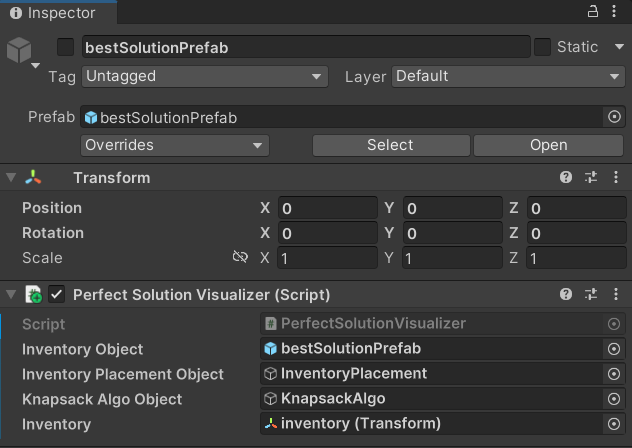
\includegraphics[scale=0.8]{images/bestSolPref_Editor}
    \caption{bestSolutionPrefab im Unity Editor}
    \label{fig:bestSol_Editor}
\end{figure}

In der Abbildung \ref{fig:bestSol_Editor} ist das \textit{bestSolutionPrefab} um Unity Editor zu sehen. Hier können verschiedene
Einestellungen vorgenommen werden, darunter die Ebene, in der dieses Objekt liegt, die Koordinaten des Objekts im
Unity Editor selbst und die angehängte Komponente \textit{PerfectSolutionVisualizer.cs}. Zudem sind vordefinierte Werte für
bestimmte Variablen sichtbar. Diese Variablen umfassen:
\begin{itemize}
    \item \textbf{Inventory Object:} Eine Referenz auf das Prefab für die perfekte Lösung.
    \item \textbf{Inventory Placement Object:} Eine Referenz auf das \textit{inventoryPlacement} Game Objekt.
    \item \textbf{Knapsack Algo Object:} Eine Referenz auf das \textit{KnapsackAlgo} Game Objekt.
    \item \textbf{Inventory:} Eine Referenz auf das \textit{Inventory} Modell, welches in dem Best Solution Prefab enthalten ist
\end{itemize}

\begin{figure}[h]
    \centering
    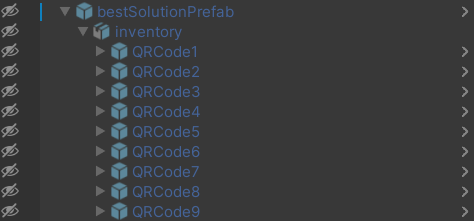
\includegraphics[scale=0.8]{images/bestSolPref}
    \caption{Inventar Prefab Hirarchie im Unity Editor}
    \label{fig:InvPref}
\end{figure}

Abbildung \ref{fig:InvPref} zeigt den Aufbau beziehungsweise die Hirarchie des Prefabs für die perfekte Lösung. Hier ist
zu sehen, dass in dem Haupt Game Objekt das Game Objekt \textit{Inventory} untergeordnet ist. Dieses Game Objekt ist
das 3D-Modell für das Inventars. Zusätzlich hat dieses \textit{Inventory}-Game Objekt mehrere Untergeordnete Prefabs.
Diese \textit{QRItem}-Prefabs sind wichtig um anhand der \textit{ID} das richtige Modell anzuzeigen. Dieses Das Gesamt-Prefab
sieht dann im Unity-Editor folgendermaßen aus:
\begin{figure}[h]
    \centering
    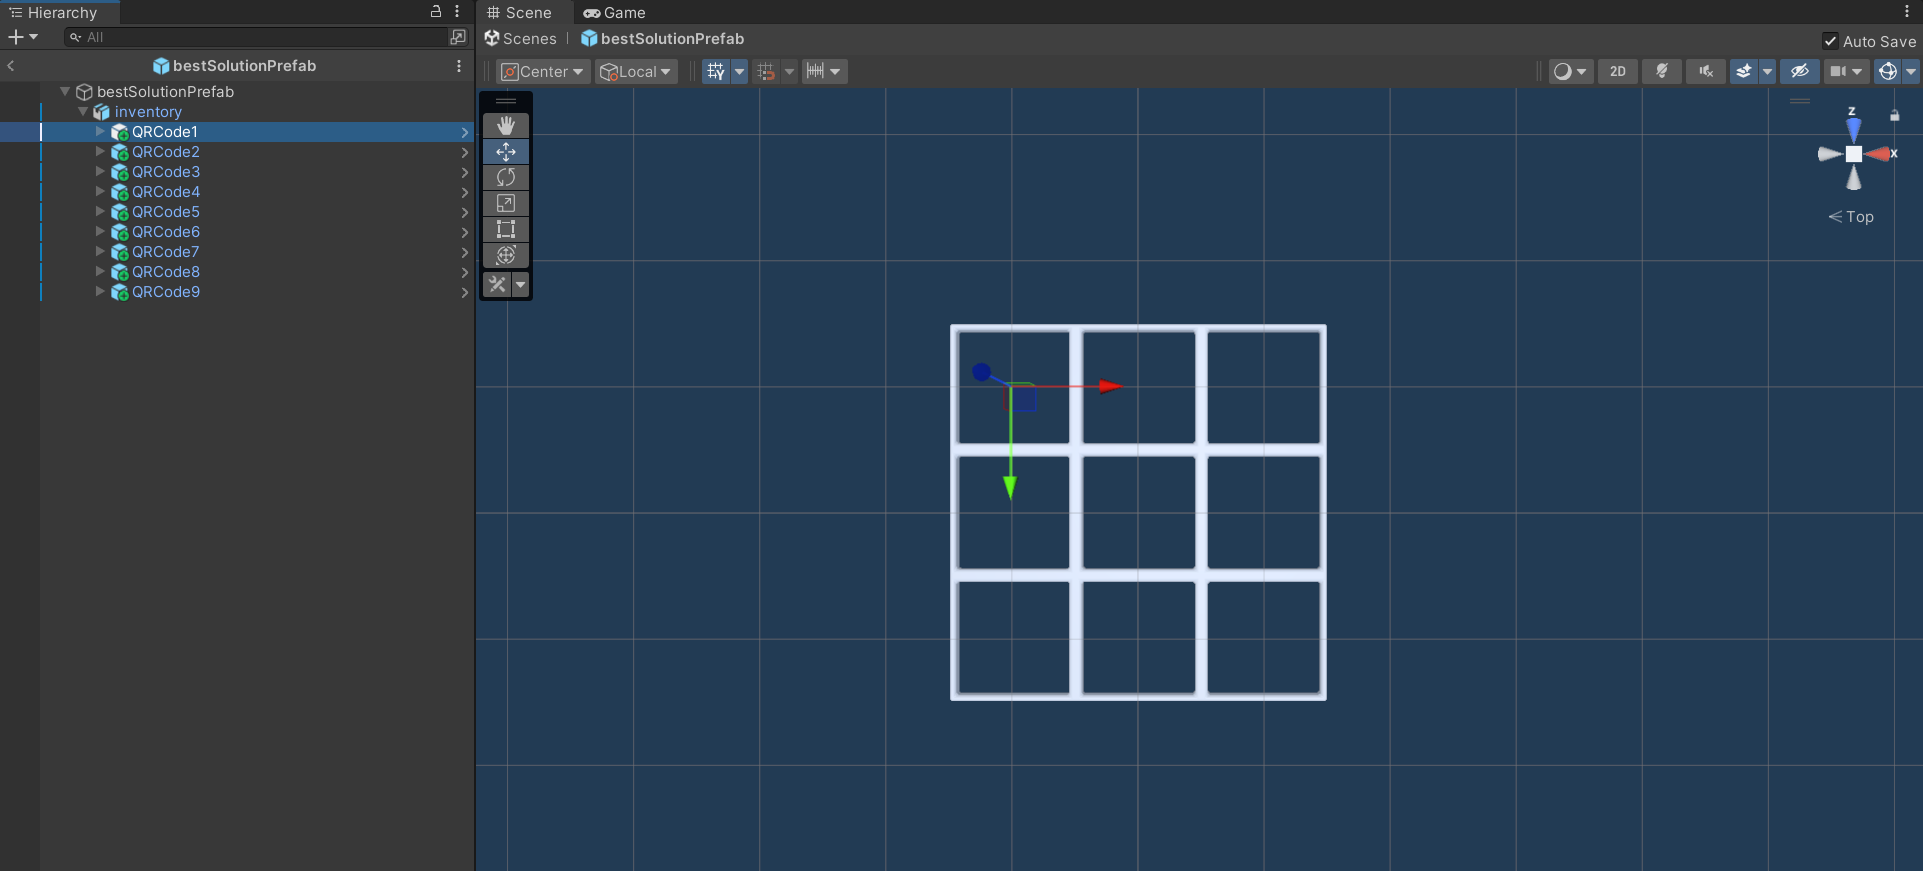
\includegraphics[scale=0.3]{images/prefShow}
    \caption{Inventar Prefab im Unity Editor}
    \label{fig:InvPrefUn}
\end{figure}

In dieser Abbildung ist zu sehen, dass das \textit{QRItem1}-Prefab in der linken oberen Ecke platziert ist. Weitergehend
ist jedes der \textit{QRItems} in einer Zelle des Inventars platziert um dann später anhand eines \textit{Indexes} das
\textit{Array} in dem die perfekte Lösung gespeichert ist zu durchlaufen um dann tatsächlich die zugehörigen Modelle
in dem zugehörigen \textit{QRItem} zu aktivieren und anzuzeigen.

\subsubsection{Script aufruf}
Um die perfekte Lösung anzuzeigen, wird das Skript \textit{PerfectSolutionVisualizer.cs} durch Betätigen eines Knopfes
aufgerufen. Der zugehörige Knopf, der das Auslösen dieses Skripts bewirkt, ist im Objekt \textit{infoObject} enthalten.
Der Aufruf dieses Skripts ist in der folgenden Abbildung dargestellt:
\begin{figure}[h]
    \centering
    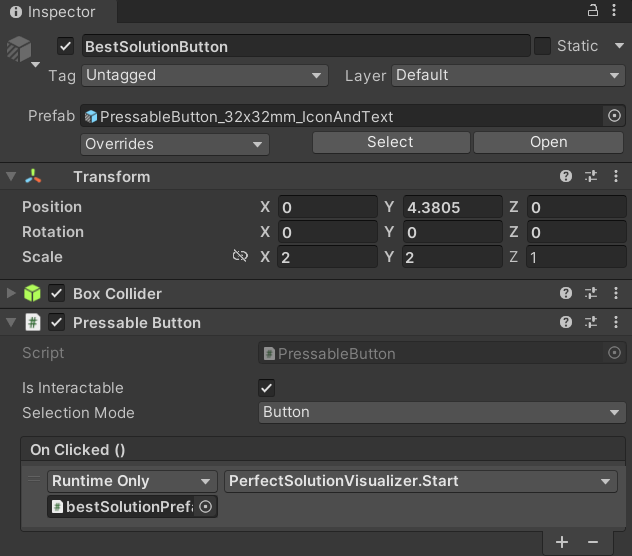
\includegraphics[scale=0.8]{images/perfSolBut}
    \caption{Script Aufruf bei Knopfdruck}
    \label{fig:ScrAuf}
\end{figure}

In Abbildung \ref{fig:ScrAuf} sind die Komponenten des \textit{BestSolutionButton} zu sehen. Der wesentliche Teil dieser
Abbildung ist das Skript \textit{PressableButton}. Dieses Skript stellt die Funktion \textbf{OnClicked()} zur Verfügung,
die einen einfachen Knopfdruck implementiert. In dieser Funktion wird in diesem Fall die \textit{Start()}-Funktion des
Skripts \textit{PerfectSolutionVisualizer.cs} aufgerufen, um das Skript zu starten.

\subsubsection{Klassenvariablen PerfectSolutionVisualizer}
\begin{lstlisting}[style=csharp, caption={Klassenvariablen des PerfectSolutionVisualizer}, label=code:Klassenvariablen_PSV]
public GameObject inventoryObject;
public GameObject inventoryPlacementObject;
public GameObject KnapsackAlgoObject;
public Transform inventory;

private PlaceObjectOnLookedAtDesk anchorScript;
private KnapsackScript knapsackScript;
private Vector3 originalInventoryPosition;
private int[,] perfectSolution;
private bool isClicked = false;
private int numRows = 3;
private int numColumns = 3;
\end{lstlisting}\\
Im Codeabschnitt \ref{code:Klassenvariablen_PSV} sind die Klassenvariablen der Klasse \textit{PerfectSolutionVisualizer}
aufgeführt. Öffentliche (\textbf{public}) Variablen repräsentieren Objekte und Werte, die im Unity Editor festgelegt und
übergeben werden oder von anderen Klassen für die Funktionalität benötigt werden. Diese Bereitstellung ermöglicht einen
direkten Zugriff auf diese Objekte in der eigenen oder einer anderen Klasse.

Besonders wichtig ist der Zugriff auf die Variablen \textit{inventoryPlacementObject} und \textit{KnapsackAlgoObject},
um im weiteren Verlauf dieses Skripts auf die beiden angehängten Skripte dieser Game-Objekte zuzugreifen. Diese Skripte
speichern die Position des Inventars und das \textit{usedItems}-Array, die für die Anzeige der perfekten Lösung benötigt
werden. Die Position des originalen Inventars ist notwendig, um die perfekte Lösung korrekt zu platzieren, während das
\textit{usedItems}-Array später benötigt wird, um das \textit{bestSolutionPrefab} anhand der gespeicherten Werte zu befüllen.

\subsubsection{Start des PerfectSolutionVisualizer}
\begin{lstlisting}[style=csharp, caption={PerfectSolutionVisualizer Start}, label=code:Start_PSV]
public void Start()
{
    isClicked = !isClicked;
    if (isClicked == true)
        {
        anchorScript = inventoryPlacementObject.GetComponent<PlaceObjectOnLookedAtDesk>();
        originalInventoryPosition = anchorScript.objectPosition;
        knapsackScript = KnapsackAlgoObject.GetComponent<KnapsackScript>();
        perfectSolution = knapsackScript.usedItems;
        printItems();
        setNewPosition();
        inventoryObject.SetActive(true);
        fillInventory();
    }
    else
        {
        inventoryObject.SetActive(false);
    }
}
\end{lstlisting}\\
Im Codeabschnitt (\ref{code:Start_PSV}) wird die Lebenszyklusmethode \textbf{Start()} aufgerufen, die bei einem Knopfdruck
ausgeführt wird. Innerhalb dieser Funktion wird zunächst die Klassenvariable \textit{isClicked} negiert, um sicherzustellen,
dass bei erneutem Klicken des Knopfes das Objekt deaktiviert wird und die Lösung nicht mehr sichtbar ist.

Falls \textit{isClicked} true ist, werden anschließend die \textit{objectPosition} der Klasse \textit{PlaceObjectOnLookedAtDesk}
und das \textit{usedItems}-Array der Klasse \textit{KnapsackScript} gespeichert. Im weiteren Verlauf werden dann die
Funktionen \textbf{setNewPosition()} und \textbf{fillInventory()} aufgerufen. Die genauen Details dieser beiden Funktionen
werden in den folgenden beiden Abschnitten näher erläutert.

\subsubsection{Setzen der neuen Position der perfekten Lösung}
\begin{lstlisting}[style=csharp, caption={Neue Position setzen}, label=code:newPos_PSV]
private void setNewPosition()
{
    Vector3 newPosition = originalInventoryPosition + Vector3.forward * 0.5f + Vector3.up * 0.205f;
    inventoryObject.transform.position = newPosition;
    Quaternion objectRotation = Quaternion.Euler(-45f, 0f, 0f);
    inventoryObject.transform.rotation = objectRotation;
}
\end{lstlisting}\\
Die im Codeabschnitt \ref{code:Start_PSV} aufgerufene Funktion \textbf{setNewPosition()} spielt eine entscheidende Rolle
für die korrekte Platzierung der perfekten Lösung. Um dieses Ziel zu erreichen, wird die ursprüngliche Position des
Inventars verwendet. Anschließend wird durch das Hinzufügen von Vektoren die Position der perfekten Lösung so angepasst,
dass sie direkt an das originale Inventar angrenzt.

\subsubsection{Perfekte Lösung füllen}
Die Funktion \textbf{fillInventory()} die nach Aktivierung des Inventars in Codeabschnitt \ref{code:Start_PSV} aufgerufen
wird ist dafür verantwortlich, dass das die korrekten Modelle des zugehörigen \textit{QRItem}-Prefabs aktiviert
und dadurch auch angezeigt wird.

\begin{lstlisting}[style=csharp, caption={Inventar füllen}, label=code:invFül_PSV]
private void fillInventory()
{
    for (int i = 0; i < numRows; i++)
    {
        for (int j = 0; j < numColumns; j++)
        {
            int id = perfectSolution[i, j];
            if (perfectSolution[i, j] == 0)
                continue;
            else
            {
                string qrCodeName = "QRCode" + (i * numColumns + j + 1);
                Transform qrCodeTransform = inventory.Find(qrCodeName);
                if (qrCodeTransform != null)
                {
                    Transform childTransform = qrCodeTransform.Find(id.ToString());
                    Debug.Log(childTransform.name);
                    if (childTransform != null)
                    {
                        childTransform.gameObject.SetActive(true);
                    }
                    else
                    {
                        Debug.LogError($"Child with id {id} not found in QRCode {qrCodeName}");
                    }
                }
                else
                {
                    Debug.LogError($"QRCode {qrCodeName} not found in the inventory");
                }
            }
        }
    }
}
\end{lstlisting}\\
Die Funktion \texttt{fillInventory()} durchläuft ein 2D-Array \texttt{perfectSolution}, das vermutlich die Lösung für
das Inventar repräsentiert. Zu Beginn wird der Wert an der Stelle $[i, j]$ des Arrays abgerufen und für spätere Verwendung
gespeichert. An jeder Position $[i, j]$ wird zunächst überprüft, ob der Wert im \texttt{perfectSolution}-Array gleich $0$
ist oder eine andere Zahl enthält. Im Fall, dass der Wert $0$ ist, wird die Schleife mit \texttt{continue} übersprungen,
da die \textit{ID: 0} darauf hinweist, dass diese Stelle im Array leer ist.

Wenn der Wert an der Stelle $[i, j]$ größer als Null ist, bedeutet dies, dass anhand dieser gespeicherten ID das
entsprechende \textit{QRItem} anhand des Namens und des darin enthaltenen Modells gefunden werden muss. Um das passende
\textit{QRItem} zu identifizieren, wird der String \texttt{QRCode} durch die Berechnung $i \times \text{numColumns} + j + 1$
zusammengesetzt. Dadurch wird anhand der Position $[i, j]$ das zugehörige \textit{QRItem} bestimmt.\\

\textbf{Beispiel:}
Angenommen in der Schleife hat $i$ den Wert $1$ und $j$ den Wert $1$. Dies bedeutet, dass das Array momentan an der Stelle $[1, 1]$
steht. Das \texttt{bestSolutionPrefab} ist so strukturiert, dass der Index nicht mit $0$, sondern mit $1$ beginnt. Daher
wird in der Berechnung am Ende $+ 1$ hinzugefügt, um dies zu berücksichtigen. Somit wird an der Stelle $[i, j]$ das
\textit{QRItem5} dem Array zugeordnet.\\

Nachdem das richtige \textit{QRItem} identifiziert wurde, wird das untergeordnete Element mit dem gefundenen Namen im
\texttt{inventory} gespeichert. Wenn dieses Objekt ungleich Null ist, ist sichergestellt, dass das Objekt existiert.
Anschließend wird nach dem Objekt mit der zu Beginn des Schleifendurchlaufs gespeicherten \textit{ID} im Kontext des
gefundenen \textit{QRItem}s gesucht. Wenn dieses Objekt existiert, wird es aktiviert, um es im Inventar anzuzeigen.
Andernfalls wird eine Fehlermeldung in die Logdatei geschrieben.

\subsection{Unit-Tests}
Durch Hilfe von Unit-Tests wird versichert, dass der implementierte Knappsack-Algorithmus
richtig und performant funktioniert.
%Genauere Erklärung + Custom Code der UnitTests

\section{Performance und Qualtitätssicherung}
\subsection{Unit-Tests}
Unit-Tests sind ein wichtiger Bestandteil der Qualitätssicherung. Sie ermöglichen die Überprüfung der korrekten
Funktionalität einzelner Komponenten und stellen sicher, dass sie wie erwartet arbeiten. Im Rahmen dieses Projekts wurden
Unit-Tests verwendet, um den Knapsack-Algorithmus zu überprüfen.  Die Tests wurden mithilfe des Unity Test Frameworks
erstellt und ausgeführt. Dieses Tool wurde speziell für die Erstellung und Ausführung von Unit-Tests in Unity entwickelt.
Durch die sorgfältige Gestaltung der Tests wurde sichergestellt, dass der Algorithmus nicht nur die erwarteten Ergebnisse
zurückgibt, sondern auch die vorgegebene Laufzeit einhält. Die Tests wurden innerhalb der Entwicklungsumgebung von Unity
durchgeführt. Die Ergebnisse wurden genau überwacht, um sicherzustellen, dass der Algorithmus zuverlässig funktioniert.

\subsection{Unity Test Framework}
Das Unity Test Framework bietet eine breite Palette von Funktionen, mit denen Entwickler umfassende Tests für ihre
Unity-Skripte schreiben und ausführen können. Dabei können verschiedene Aspekte der Skripte auf ihre korrekte Funktionalität
überprüft werden. Dazu gehören das Testen von Variablen, das Aufrufen von Funktionen und das Überprüfen von erwarteten
Ergebnissen. Entwickler können dank dieser umfangreichen Funktionen sicherstellen, dass ihre Unity-Anwendungen robust
und zuverlässig sind. So schaffen sie eine solide Grundlage für die Qualitätssicherung.

\subsection{Performance-Messung}
Die Performance des Knapsack-Algorithmus wurde mithilfe von Unit-Tests überprüft. Dabei wurde die Laufzeit des Algorithmus
für verschiedene Eingabegrößen gemessen. Die Ergebnisse wurden sorgfältig analysiert, um sicherzustellen, dass der Algorithmus
die erwartete Laufzeit einhält. Es wurden verschiedene Algorithmen und Implementierungen getestet, um die optimale
Leistung zu erzielen. Die Ergebnisse der Performance-Messung wurden genau überwacht, um sicherzustellen, dass der
Algorithmus zuverlässig und effizient arbeitet.

\begin{lstlisting}[style=csharp, caption={Inventar füllen}, label=code:invFül_PSV]
public class AlgoTest
{
    GameObject testObject;
    KnapsackScript knapsackScript;
    int[,] usedItems;
    int capacity = 120;

    [SetUp]
    public void Setup()
    {
        // Vor jedem Test eine Instanz von KnapsackScript erstellen
        testObject = new GameObject();
        knapsackScript = testObject.AddComponent<KnapsackScript>();
    }

    [TearDown]
    public void Teardown()
    {
        // Das Test-GameObject nach jedem Test zerstören
        GameObject.DestroyImmediate(testObject);
    }

    // Ein Test verhält sich wie eine normale Methode
    [Test]
    public void KnapsackMaxValue_ReturnsCorrectValue()
    {
        // Gibt eine Menge von Gegenständen für den Rucksack an
        Dictionary<int, QRData> items = new Dictionary<int, QRData>() {
        {1, new QRData { id = 1, weight = 50, value = 100 }},
        {2, new QRData { id = 2, weight = 25, value = 50 }},
        {3, new QRData { id = 3, weight = 20, value = 30 }},
        {4, new QRData { id = 4, weight = 10, value = 15 }},
        {5, new QRData { id = 5, weight = 10, value = 5 }},
        {6, new QRData { id = 6, weight = 25, value = 50 }},
        {7, new QRData { id = 7, weight = 10, value = 10 }},
        {8, new QRData { id = 8, weight = 5, value = 50 }},
        {9, new QRData { id = 9, weight = 5, value = 15 }},
        {10, new QRData { id = 10, weight = 20, value = 15 }},
        };

        System.Random random = new System.Random();
        for (int i = 11; i <= 100; i++)
        {
        int randomWeight = random.Next(1, 51);
        int randomValue = random.Next(1, 101);

        items.Add(i, new QRData { id = i, weight = randomWeight, value = randomValue });
        }

        knapsackScript.capacity = capacity;
        knapsackScript.maxItems = items.Count;
        knapsackScript.items = items;

        // Messung der Ausführungszeit für KnapsackMaxValue
        System.Diagnostics.Stopwatch knapsackMaxValueStopwatch = System.Diagnostics.Stopwatch.StartNew();
        int maxValue = knapsackScript.KnapsackMaxValue(out usedItems);
        knapsackMaxValueStopwatch.Stop();
        Debug.Log($"Die Ausführungszeit von KnapsackMaxValue beträgt: {knapsackMaxValueStopwatch.ElapsedMilliseconds} ms");

        // Messung der Ausführungszeit für KnapsackMaxValueRecursive
        System.Diagnostics.Stopwatch recursiveStopwatch = System.Diagnostics.Stopwatch.StartNew();
        int maxValueComp = KnapsackMaxValueRecursive(items.Count, capacity, items, new Dictionary<(int, int), int>());
        recursiveStopwatch.Stop();
        Debug.Log($"Die Ausführungszeit von KnapsackMaxValueRecursive beträgt: {recursiveStopwatch.ElapsedMilliseconds} ms");

        // Überprüfen, ob die Werte übereinstimmen
        Assert.AreEqual(maxValueComp, maxValue);
    }

    // Ein UnityTest verhält sich wie ein Coroutine im Play Mode. Im Edit Mode kann `yield return null;` verwendet werden, um einen Frame zu überspringen.
    [UnityTest]
    public IEnumerator AlgoTestWithEnumeratorPasses()
    {
        // Die Assert-Klasse wird verwendet, um Bedingungen zu testen.
        // Verwende yield, um einen Frame zu überspringen.
        yield return null;
    }

    // Rekursive Implementierung des Knapsack-Algorithmus zur Berechnung des maximalen Werts
    public int KnapsackMaxValueRecursive(int n, int remainingCapacity, Dictionary<int, QRData> items, Dictionary<(int, int), int> memo)
    {
        if (n == 0 || remainingCapacity == 0)
            return 0;

        if (memo.TryGetValue((n, remainingCapacity), out int memoizedValue))
            return memoizedValue;

        if (items[n].weight > remainingCapacity)
        {
            memo[(n, remainingCapacity)] = KnapsackMaxValueRecursive(n - 1, remainingCapacity, items, memo);
            return memo[(n, remainingCapacity)];
        }

        int includedValue = items[n].value + KnapsackMaxValueRecursive(n - 1, remainingCapacity - items[n].weight, items, memo);
        int excludedValue = KnapsackMaxValueRecursive(n - 1, remainingCapacity, items, memo);

        int result = Math.Max(includedValue, excludedValue);

        memo[(n, remainingCapacity)] = result;

        return result;
    }
}
\end{lstlisting}\\

%TODO Beschreibung der Unit-Tests

%Performance-Messung
